%\PassOptionsToPackage{table}{xcolor}
% \documentclass[smaller, dvipsnames,%handout,
% hyperref={colorlinks=true,urlcolor=magenta,citecolor=cyan,linkcolor=orange}]{beamer}
% \def\bmode{2} % Mode 0 for presentation, mode 1 for a handout with notes, mode 2 fo% r handout without notes
% \if 0\bmode
% \documentclass[usenames,dvipsnames,smaller]{beamer}
% \else \if 1\bmode
% \immediate\write18{pdflatex -jobname=\jobname-Handout-Notes\space\jobname}
% \documentclass[usenames,dvipsnames,smaller,handout]{beamer}
% \usepackage{handoutWithNotes}
% \pgfpagesuselayout{2 on 1 with notes}[letterpaper, landscape, border shrink=4mm]
% \else \if 2\bmode
% \immediate\write18{pdflatex -jobname=\jobname-Handout\space\jobname}
% \documentclass[usenames,dvipsnames,smaller,handout]{beamer}
% \fi
% \fi
% \fi
\documentclass[usenames,dvipsnames,smaller%,handout
]{beamer}



% \documentclass[smaller,handout
% ]{beamer}
%\usepackage{etex}
%\newcommand{\num}{6{} }

% \usetheme[
%   outer/progressbar=foot,
%   outer/numbering=counter,
%  block=fill
% ]{metropolis}

%\useoutertheme{metropolis}

\usetheme{Madrid}
\useoutertheme[subsection=false]{miniframes} % Alternatively: miniframes, infolines, split
\useinnertheme{circles}
\usecolortheme{seahorse}

\usepackage[backend=biber,style=authoryear,maxcitenames=2,maxbibnames=99,safeinputenc,url=false,
eprint=false]{biblatex}
\addbibresource{bib/references.bib}
\AtEveryCitekey{\iffootnote{{\tiny}\tiny}{\tiny}}

%\usepackage{pgfpages}
%\setbeameroption{hide notes} % Only slides
%\setbeameroption{show only notes} % Only notes
%\setbeameroption{hide notes} % Only notes
%\setbeameroption{show notes on second screen=right} % Both

% \usepackage[sfdefault]{Fira Sans}

% \setsansfont[BoldFont={Fira Sans}]{Fira Sans Light}
% \setmonofont{Fira Mono}

%\usepackage{fira}
%\setsansfont{Fira}
%\setmonofont{Fira Mono}
% To give a presentation with the Skim reader (http://skim-app.sourceforge.net) on OSX so
% that you see the notes on your laptop and the slides on the projector, do the following:
% 
% 1. Generate just the presentation (hide notes) and save to slides.pdf
% 2. Generate onlt the notes (show only nodes) and save to notes.pdf
% 3. With Skim open both slides.pdf and notes.pdf
% 4. Click on slides.pdf to bring it to front.
% 5. In Skim, under "View -> Presentation Option -> Synhcronized Noted Document"
%    select notes.pdf.
% 6. Now as you move around in slides.pdf the notes.pdf file will follow you.
% 7. Arrange windows so that notes.pdf is in full screen mode on your laptop
%    and slides.pdf is in presentation mode on the projector.

% Give a slight yellow tint to the notes page
%\setbeamertemplate{note page}{\pagecolor{yellow!5}\insertnote}\usepackage{palatino}


%\usetheme{metropolis}
%\usecolortheme{beaver}
%\usepackage{xcolor}
\definecolor{darkcandyapplered}{HTML}{A40000}
\definecolor{lightcandyapplered}{HTML}{e74c3c}

%\setbeamercolor{title}{fg=darkcandyapplered}
%\setbeamercolor{frametitle}{bg=darkcandyapplered!80!black!90!white}
%\setbeamertemplate{frametitle}{\bf\insertframetitle}
%\setbeamercolor{footnote mark}{fg=darkcandyapplered}
%\setbeamercolor{footnote}{fg=darkcandyapplered!70}
%\Raggedbottom
%\setbeamerfont{page number in head/foot}{size=\tiny}
%\usepackage[tracking]{microtype}


\setbeamertemplate{frametitle}{%
    \nointerlineskip%
    \begin{beamercolorbox}[wd=\paperwidth,ht=2.0ex,dp=0.6ex]{frametitle}
        \hspace*{1ex}\insertframetitle%
    \end{beamercolorbox}%
}



\setbeamerfont{caption}{size=\footnotesize}
\setbeamercolor{caption name}{fg=darkcandyapplered}


%\usepackage[sc,osf]{mathpazo}   % With old-style figures and real smallcaps.
%\linespread{1.025}              % Palatino leads a little more leading

% Euler for math and numbers
%\usepackage[euler-digits,small]{eulervm}
%\AtBeginDocument{\renewcommand{\hbar}{\hslash}}
\usepackage{graphicx,multirow,paralist,booktabs}


%\mode<presentation> { \setbeamercovered{transparent} }

\setbeamertemplate{navigation symbols}{}
\makeatletter
\def\beamerorig@set@color{%
  \pdfliteral{\current@color}%
  \aftergroup\reset@color
}
\def\beamerorig@reset@color{\pdfliteral{\current@color}}
\makeatother

%=== GRAPHICS PATH ===========
\graphicspath{{./m3-images/}}
% Marginpar width
%Marginpar width
%\setlength{\marginparsep}{.02in}


%% Captions
% \usepackage{caption}
% \captionsetup{
%   labelsep=quad,
%   justification=raggedright,
%   labelfont=sc
% }

%AMS-TeX packages

\usepackage{amssymb,amsmath,amsthm} 
\usepackage{bm}
\usepackage{color}

\usepackage{hyperref,enumerate}
\usepackage{minitoc,array}


%https://tex.stackexchange.com/a/31370/2269
\usepackage{mathtools,cancel}

\renewcommand{\CancelColor}{\color{red}} %change cancel color to red

\makeatletter
\let\my@cancelto\cancelto %copy over the original cancelto command
\newcommand<>{\cancelto}[2]{\alt#3{\my@cancelto{#1}{#2}}{\mathrlap{#2}\phantom{\my@cancelto{#1}{#2}}}}
% redefine the cancelto command, using \phantom to assure that the
% result doesn't wiggle up and down with and without the arrow
\makeatother


\definecolor{slblue}{rgb}{0,.3,.62}
\hypersetup{
    colorlinks,%
    citecolor=blue,%
    filecolor=blue,%
    linkcolor=blue,
    urlcolor=slblue
}

%%%TIKZ
\usepackage{tikz}
\usepackage{pgfplots}
\usepackage{pgfplotstable}
\usepackage{pgfgantt}
\usepackage{tikzsymbols}
\pgfplotsset{compat=newest}

\usetikzlibrary{arrows,shapes,positioning,shapes.geometric}
\usetikzlibrary{decorations.markings}
\usetikzlibrary{shadows,automata}
\usetikzlibrary{patterns}
\usetikzlibrary{trees,mindmap,backgrounds}
%\usetikzlibrary{circuits.ee.IEC}
\usetikzlibrary{decorations.text}
% For Sagnac Picture
\usetikzlibrary{%
    decorations.pathreplacing,%
    decorations.pathmorphing%
}
\tikzset{no shadows/.style={general shadow/.style=}}
%
%\usepackage{paralist}


%%% FORMAT PYTHON CODE
%\usepackage{listings}
% Default fixed font does not support bold face
\DeclareFixedFont{\ttb}{T1}{txtt}{bx}{n}{8} % for bold
\DeclareFixedFont{\ttm}{T1}{txtt}{m}{n}{8}  % for normal

% Custom colors
\definecolor{deepblue}{rgb}{0,0,0.5}
\definecolor{deepred}{rgb}{0.6,0,0}
\definecolor{deepgreen}{rgb}{0,0.5,0}

\usepackage{listings}

% Python style for highlighting
\newcommand\pythonstyle{\lstset{
language=Python,
basicstyle=\footnotesize\ttm,
otherkeywords={self},             % Add keywords here
keywordstyle=\footnotesize\ttb\color{deepblue},
emph={MyClass,__init__},          % Custom highlighting
emphstyle=\footnotesize\ttb\color{deepred},    % Custom highlighting style
stringstyle=\color{deepgreen},
frame=tb,                         % Any extra options here
    showstringspaces=false            % 
}}

% % Python environment
\lstnewenvironment{python}[1][]
{
\pythonstyle
\lstset{#1}
}
{}

% % Python for external files
% \newcommand\pythonexternal[2][]{{
% \pythonstyle
% \lstinputlisting[#1]{#2}}}

% Python for inline
% 
\newcommand\pythoninline[1]{{\pythonstyle\lstinline!#1!}}


\newcommand{\osn}{\oldstylenums}
\newcommand{\dg}{^{\circ}}
\newcommand{\lt}{\left}
\newcommand{\rt}{\right}
\newcommand{\pt}{\phantom}
\newcommand{\tf}{\therefore}
\newcommand{\?}{\stackrel{?}{=}}
\newcommand{\fr}{\frac}
\newcommand{\dfr}{\dfrac}
\newcommand{\ul}{\underline}
\newcommand{\tn}{\tabularnewline}
\newcommand{\nl}{\newline}
\newcommand\relph[1]{\mathrel{\phantom{#1}}}
\newcommand{\cm}{\checkmark}
\newcommand{\ol}{\overline}
\newcommand{\rd}{\color{red}}
\newcommand{\bl}{\color{blue}}
\newcommand{\pl}{\color{purple}}
\newcommand{\og}{\color{orange!90!black}}
\newcommand{\gr}{\color{green!40!black}}
\newcommand{\nin}{\noindent}
\newcommand{\la}{\lambda}
\renewcommand{\th}{\theta}
\newcommand{\al}{\alpha}
\newcommand{\G}{\Gamma}
\newcommand*\circled[1]{\tikz[baseline=(char.base)]{
            \node[shape=circle,draw,thick,inner sep=1pt] (char) {\small #1};}}

\newcommand{\bc}{\begin{compactenum}[\quad--]}
\newcommand{\ec}{\end{compactenum}}

\newcommand{\p}{\partial}
\newcommand{\pd}[2]{\frac{\partial{#1}}{\partial{#2}}}
\newcommand{\dpd}[2]{\dfrac{\partial{#1}}{\partial{#2}}}
\newcommand{\pdd}[2]{\frac{\partial^2{#1}}{\partial{#2}^2}}


\pgfmathdeclarefunction{poiss}{1}{%
  \pgfmathparse{(#1^x)*exp(-#1)/(x!)}%
  }

\pgfmathdeclarefunction{gauss}{2}{%
  \pgfmathparse{1/(#2*sqrt(2*pi))*exp(-((x-#1)^2)/(2*#2^2))}%
}

\makeatletter
\long\def\ifnodedefined#1#2#3{%
    \@ifundefined{pgf@sh@ns@#1}{#3}{#2}%
}

\pgfplotsset{
    discontinuous/.style={
    scatter,
    scatter/@pre marker code/.code={
        \ifnodedefined{marker}{
            \pgfpointdiff{\pgfpointanchor{marker}{center}}%
             {\pgfpoint{0}{0}}%
             \ifdim\pgf@y>0pt
                \tikzset{options/.style={mark=*, fill=white}}
                \draw [densely dashed] (marker-|0,0) -- (0,0);
                \draw plot [mark=*] coordinates {(marker-|0,0)};
             \else
                \tikzset{options/.style={mark=none}}
             \fi
        }{
            \tikzset{options/.style={mark=none}}        
        }
        \coordinate (marker) at (0,0);
        \begin{scope}[options]
    },
    scatter/@post marker code/.code={\end{scope}}
    }
}

\makeatother

%%%%%%%%%%%%%%%%%%%%%%%%%%%%%%%%%%%%%%%%%%%%%%%%%%%
%%%%%%%%%%%%%%%%%%%%%%%%%%%%%%%%%%%%%%%%%%%%%%%%%%%

\title[CEE 260/MIE 273 Lecture 3B: Normal Distribution]{{\normalsize CEE 260/MIE 273: Probability and Statistics in Civil Engineering} \\
Lecture 3B: The Normal Distribution}
\date[September 25, 2025]{\footnotesize September 25, 2025}
\author{{\bf Prof.\ Oke}}
\institute[UMass Amherst]{
  \begin{tikzpicture}[baseline=(current bounding box.center)]
    \node[anchor=base] at (-7,0) (its) {
\includegraphics[scale=.3]{UMassEngineering_vert}} ;
  \end{tikzpicture}
}



%https://tex.stackexchange.com/questions/55806/mindmap-tikzpicture-in-beamer-reveal-step-by-step
  % \tikzset{
  %   invisible/.style={opacity=0},
  %   visible on/.style={alt={#1{}{invisible}}},
  %   alt/.code args={<#1>#2#3}{%
  %     \alt<#1>{\pgfkeysalso{#2}}{\pgfkeysalso{#3}} % \pgfkeysalso doesn't change the path
  %   },
  % }


\usepackage{listings}

\lstset{language=matlab,
                basicstyle=\scriptsize\ttfamily,
                keywordstyle=\color{blue}\ttfamily,
                stringstyle=\color{blue}\ttfamily,
                commentstyle=\color{gray}\ttfamily,
                morecomment=[l][\color{gray}]{\#}
              }
         
\begin{document}

\maketitle




\begin{frame}
  \frametitle{Outline}
  \tableofcontents

  Reading: OpenIntro Statistics 4.1
\end{frame}



 


% \begin{frame}
%   \frametitle{Relationship between binomial and normal distributions (cont.)} \pause
%   Consider the distribution $B(n=20,p=0.6)$. \pause

%   We see that it can be approximated by $N(\mu = np, \sigma^2 = npq)$. \pause

%   \begin{tikzpicture}[
%     declare function={binom(\k,\n,\p)=\n!/(\k!*(\n-\k)!)*\p^\k*(1-\p)^(\n-\k);}
%     ]
%     \begin{axis}[
%       samples at={0,...,20},
%       xlabel=$x$,
%       ylabel=$P(x)$,
%       xlabel style={right},
%       ylabel style={above left},
%       xtick={0,20,...,100},
% %      ytick={0.05,0.1,0.15},
%       axis x line=center,
%       axis y line=center,
%       xmax = 22,
%       ymax =.22,
%       y post scale = .7,
%       x post scale=1.2,
%       legend style={at={(1.25, 1)},anchor=north east},
%       yticklabel style={
%         /pgf/number format/fixed,
%         /pgf/number format/fixed zerofill,
%         /pgf/number format/precision=2
%       }
%       ]
%       \only<4->{\addplot+[ycomb,opacity=.5] {binom(x,20,0.6)}; \addlegendentry{$B(n=20,p=0.6)$}}
%       \only<5->{\addplot+[thick,samples=100,opacity=.5,no markers] {gauss(12,2.19))};}
%       \only<6->{\addlegendentry{$N(\mu =12, \sigma^2=4.8)$};}
%     \end{axis}
%   \end{tikzpicture}

  
% \end{frame}

% \begin{frame}
%   \frametitle{Relationship between binomial and normal distributions}
%   If a binomial PMF is not too skewed, then $X\sim B(n,p)$ is approximately normally distributed with $\mu = np$ and $\sigma^2 = npq$.

%   \pause

%   Thus:
%   \begin{equation}
%     \label{eq:36}
%     P(X\le x) \approx \Phi\lt( \fr{x + 0.5 -np}{\sqrt{np(1-p)}}\rt) \quad np \ge 10; n(1-p) \ge 10
%   \end{equation}
% \end{frame}


\section{The normal distribution}

\begin{frame}
  \frametitle{Normal (Gaussian) distribution}

  \begin{block}{Definition}\pause
    Denoted as $\mathcal{N}(\mu,\sigma^2)$ or $\mathcal{N}(\mu,\sigma)$, the normal distribution is continuous with PDF:

    \pause
    
    \begin{equation}
      \label{eq:1}
      f_X(x) = \fr{1}{\sigma\sqrt{2\pi}}e^{-\fr{1}{2}\lt(\fr{x-\mu}{\sigma}\rt)^2}
      \pause\equiv 
      \fr{1}{\sigma\sqrt{2\pi}}\exp\lt[{-\fr{1}{2}\lt(\fr{x-\mu}{\sigma}\rt)^2}\rt]
      \quad -\infty< x < \infty
    \end{equation}
    \pause
    
    where $\mu$ and $\sigma^2$ (or $\sigma$) are its parameters (mean and variance (or standard deviation)).
  \end{block}

  \pause
  \begin{center}
    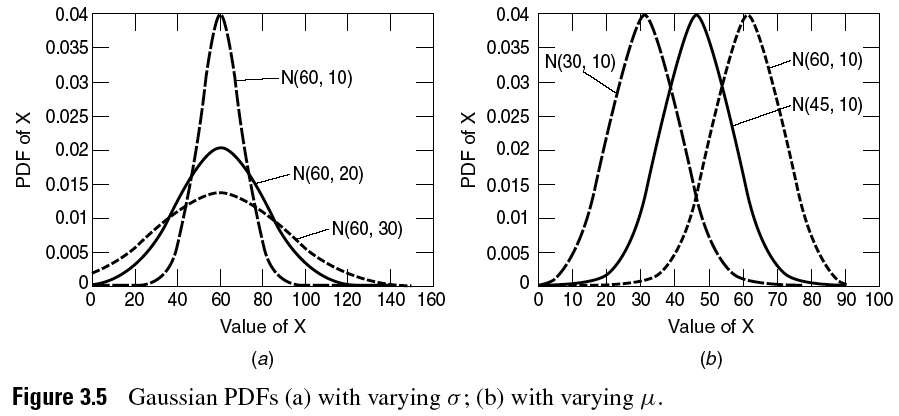
\includegraphics[width=.75\textwidth]{03_05}
  \end{center}
\end{frame}

\begin{frame}
  \frametitle{Example 1: Normal distribution parameters}
  \pause
  \begin{enumerate}[\bf (a)] \pause
  \item   A random variable $X$ is normally distributed as: $X\sim \mathcal{N}(\mu = 0,\sigma^{2}= 1)$. What are the mean and standard deviation of this distribution?
    \pause
    {\gr Mean: $\mu = 0$, standard deviation: $\sigma = 1$} \pause



  \item  A random variable $X$ is normally distributed as: $X\sim \mathcal{N}(\mu=2, \sigma^2=4)$. What are the mean and variance of this distribution? \pause
    {\gr  Mean: $\mu = 2$, variance: $\sigma^2 = 4 $} 
      \end{enumerate}

    \pause

    \begin{minipage}
      {0.48\textwidth}
          \begin{figure}[htbp]
\centering
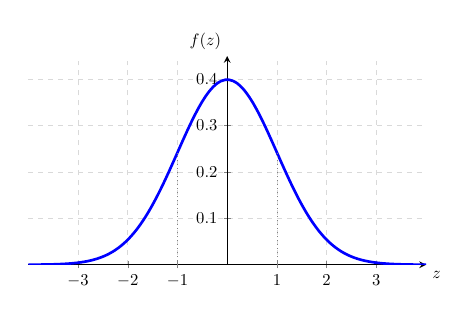
\begin{tikzpicture}[scale=.6]
\begin{axis}[
    width=10cm,
    height=6cm,
    axis lines=center,
    xlabel={$z$},
    ylabel={$f(z)$},
    xlabel style={below right},
    ylabel style={above left},
    xmin=-4, xmax=4,
    ymin=0, ymax=0.45,
    xtick={-3,-2,-1,0,1,2,3},
    ytick={0,0.1,0.2,0.3,0.4},
    grid=major,
    grid style={dashed,gray!30},
    samples=100,
    smooth,
    thick
]

% Plot the standard normal distribution
\addplot[blue, ultra thick, domain=-4:4] {1/sqrt(2*pi) * exp(-0.5*x^2)};

% Mark the mean
\draw[black, thick, dotted] (axis cs:0,0) -- (axis cs:0,{1/sqrt(2*pi)});
%\node[black, above] at (axis cs:0,{1/sqrt(2*pi) + 0.02}) {$\mu = 0$};

% Add distribution parameters
%\node[above] at (axis cs:0,0.42) {$\mathcal{N}(0, 1)$};

% Mark standard deviation points
\draw[gray, thin, dotted] (axis cs:-1,0) -- (axis cs:-1,{1/sqrt(2*pi) * exp(-0.5)});
\draw[gray, thin, dotted] (axis cs:1,0) -- (axis cs:1,{1/sqrt(2*pi) * exp(-0.5)});
%\node[gray, below] at (axis cs:-1,-0.02) {$-\sigma$};
%\node[gray, below] at (axis cs:1,-0.02) {$+\sigma$};

\end{axis}
\end{tikzpicture}
\caption{Standard normal distribution $\mathcal{N}(0, 1)$}
\label{fig:standard_normal}
\end{figure}\pause
    \end{minipage}
    \begin{minipage}
      {0.48\textwidth}          
 \begin{figure}[htbp]
\centering
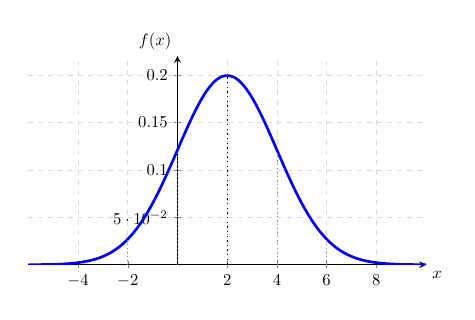
\begin{tikzpicture}[scale=.6]
\begin{axis}[
    width=10cm,
    height=6cm,
    axis lines=center,
    xlabel={$x$},
    ylabel={$f(x)$},
    xlabel style={below right},
    ylabel style={above left},
    xmin=-6, xmax=10,
    ymin=0, ymax=0.22,
    xtick={-4,-2,0,2,4,6,8},
    ytick={0,0.05,0.10,0.15,0.20},
    grid=major,
    grid style={dashed,gray!30},
    samples=100,
    smooth,
    thick
]

% Plot the normal distribution with μ=2, σ=2
\addplot[blue, ultra thick, domain=-6:10] {1/(2*sqrt(2*pi)) * exp(-0.5*((x-2)/2)^2)};

% Mark the mean
\draw[black, thick, dotted] (axis cs:2,0) -- (axis cs:2,{1/(2*sqrt(2*pi))});
%\node[black, above] at (axis cs:2,{1/(2*sqrt(2*pi)) + 0.01}) {$\mu = 2$};

% Add distribution parameters
%%\node[above] at (axis cs:2,0.205) {$\mathcal{N}(2, 2^2)$};

% Mark standard deviation points
\draw[gray, thin, dotted] (axis cs:0,0) -- (axis cs:0,{1/(2*sqrt(2*pi)) * exp(-0.5)});
\draw[gray, thin, dotted] (axis cs:4,0) -- (axis cs:4,{1/(2*sqrt(2*pi)) * exp(-0.5)});
\draw[gray, thin, dotted] (axis cs:-2,0) -- (axis cs:-2,{1/(2*sqrt(2*pi)) * exp(-2)});
\draw[gray, thin, dotted] (axis cs:6,0) -- (axis cs:6,{1/(2*sqrt(2*pi)) * exp(-2)});

% % Labels for standard deviation markers
% \node[gray, below] at (axis cs:0,-0.01) {$\mu-\sigma$};
% \node[gray, below] at (axis cs:4,-0.01) {$\mu+\sigma$};
% \node[gray, below] at (axis cs:-2,-0.01) {$\mu-2\sigma$};
% \node[gray, below] at (axis cs:6,-0.01) {$\mu+2\sigma$};

\end{axis}
\end{tikzpicture}
\caption{Normal distribution with $\mu = 2$, $\sigma = 2$}
\label{fig:normal_mu2_sigma2}
\end{figure}
\end{minipage}
\end{frame}


\begin{frame}
  \frametitle{CDF of a normal distribution}
  \pause

  \begin{itemize}[<+->]
  \item The CDF of a normal distribution is the integral of the PDF:
    \begin{equation}
      F_{X}(x) = P(X\le x) =
      \int_{-\infty}^{x} f_{x}(x)dx = \pause  \int_{-\infty}^{x}  \fr{1}{\sigma\sqrt{2\pi}}\exp\lt[{-\fr{1}{2}\lt(\fr{x-\mu}{\sigma}\rt)^2}\rt] dx
    \end{equation}
    \medskip

  \item There is no closed-form solution to this integral

    \medskip
    
  \item So, in texts/tables, we denote the \textbf{\rd standard normal} CDF as $\Phi(z)$, where:
    \begin{equation}
      \Phi(z) =   \int_{-\infty}^{z} f_{Z}(z) \fr{1}{1\sqrt{2\pi}}\exp\lt[{-\fr{1}{2}z^2}\rt] dz \pause = P(Z \le z)
    \end{equation}
    where \pause

    \begin{equation}
    z = \frac{x - \mu}{\sigma}
  \end{equation}

  \item The standardized normal variable $z$ is often referred to as the $Z$-score
  \end{itemize}
\end{frame}



\section{Standard normal distribution}
\begin{frame}
  \frametitle{Standard normal distribution}

  If a random variable $X$ has a normal distribution $\mathcal{N}(\mu,\sigma^2)$, then the r.v. $Z$ has a \alert{standard normal distribution} if

  \begin{equation}
    \label{eq:2}
    Z = \fr{X - \mu}{\sigma} \sim \mathcal{N}(0,1)
  \end{equation}

  \pause

  The {\bf standardized normal} therefore has a mean of 0 and variance of 1. \pause
  Its PDF is thus:
  
  \begin{equation}
    \label{eq:3}
    f_Z(z) = \fr{1}{\sqrt{2\pi}}e^{-\fr{1}{2}z^2} \quad -\infty < z < \infty
    \end{equation}

    \pause

    The CDF $\Phi$ of the standard normal variate $Z$ is given by:
    \begin{equation}
      \label{eq:6}
      \Phi(z) = F_Z(z) \equiv P(Z \le z)
    \end{equation}
\end{frame}

\begin{frame}
  \frametitle{Example 2: Computing the $Z$-score}
  \pause

  If $X\sim\mathcal{N}(10, \sigma^2=4)$, what is the $Z$-score of a sample $x=5$? \pause
    {\gr
      \begin{eqnarray*}
        z &=& \fr{x - \mu}{\sigma} = \pause \fr{5 - 10}{\sqrt{4}} \\\pause
        &=& -\fr{5}{2} = \boxed{-2.5}
      \end{eqnarray*}
      \pause
      This means that the sample $x=5$ is 2.5 standard deviations below the mean
      }
\pause
\begin{minipage}{.45\linewidth}
\begin{figure}[htbp]
\centering
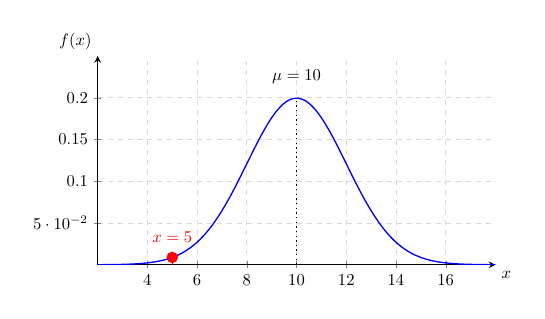
\begin{tikzpicture}[scale=.6]
\begin{axis}[
    width=10cm,
    height=6cm,
    axis lines=center,
    xlabel={$x$},
    ylabel={$f(x)$},
    xlabel style={below right},
    ylabel style={above left},
    xmin=2, xmax=18,
    ymin=0, ymax=0.25,
    xtick={4,6,8,10,12,14,16},
    ytick={0,0.05,0.10,0.15,0.20},
    grid=major,
    grid style={dashed,gray!30},
    samples=100,
    smooth,
    thick
]

% Plot the normal distribution with μ=10, σ²=4 (σ=2)
\addplot[blue, thick, domain=2:18] {1/(2*sqrt(2*pi)) * exp(-0.5*((x-10)/2)^2)};

% Mark x = 5
\addplot[red, thick, mark=*, mark size=3pt] coordinates {(5, {1/(2*sqrt(2*pi)) * exp(-0.5*((5-10)/2)^2)})};

% Draw vertical line at x = 5
\draw[red, thick, dashed] (axis cs:5,0) -- (axis cs:5,{1/(2*sqrt(2*pi)) * exp(-0.5*((5-10)/2)^2)});

% Label the point
\node[red, above] at (axis cs:5,{1/(2*sqrt(2*pi)) * exp(-0.5*((5-10)/2)^2) + 0.01}) {$x = 5$};

% Mark the mean
\draw[black, thick, dotted] (axis cs:10,0) -- (axis cs:10,{1/(2*sqrt(2*pi))});
\node[black, above] at (axis cs:10,{1/(2*sqrt(2*pi)) + 0.01}) {$\mu = 10$};

% Add title and parameters
% \node[above] at (axis cs:10,0.205) {\textbf{Normal Distribution}};
% \node[above] at (axis cs:10,0.19) {$\mu = 10, \sigma^2 = 4, \sigma = 2$};

\end{axis}
\end{tikzpicture}
\caption{Normal distribution with $\mu = 10$, $\sigma^2 = 4$, and $x = 5$ indicated}
\label{fig:normal_dist_mu10_var4_x5}
\end{figure}
\end{minipage}\pause\hfill
\begin{minipage}{.45\linewidth}
\begin{figure}[htbp]
\centering
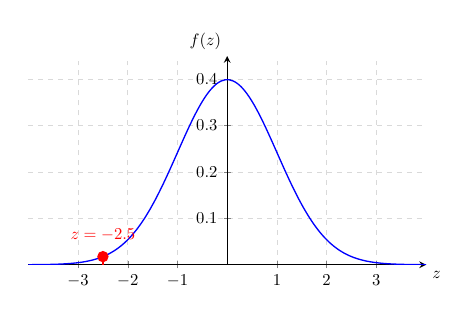
\begin{tikzpicture}[scale=.6]
\begin{axis}[
    width=10cm,
    height=6cm,
    axis lines=center,
    xlabel={$z$},
    ylabel={$f(z)$},
    xlabel style={below right},
    ylabel style={above left},
    xmin=-4, xmax=4,
    ymin=0, ymax=0.45,
    xtick={-3,-2,-1,0,1,2,3},
    ytick={0,0.1,0.2,0.3,0.4},
    grid=major,
    grid style={dashed,gray!30},
    samples=100,
    smooth,
    thick
]

% Plot the standard normal distribution
\addplot[blue, thick, domain=-4:4] {1/sqrt(2*pi) * exp(-0.5*x^2)};

% Mark z = -2.5
\addplot[red, thick, mark=*, mark size=3pt] coordinates {(-2.5, {1/sqrt(2*pi) * exp(-0.5*(-2.5)^2)})};

% Draw vertical line at z = -2.5
\draw[red, thick, dashed] (axis cs:-2.5,0) -- (axis cs:-2.5,{1/sqrt(2*pi) * exp(-0.5*(-2.5)^2)});

% Label the point
\node[red, above] at (axis cs:-2.5,{1/sqrt(2*pi) * exp(-0.5*(-2.5)^2) + 0.02}) {$z = -2.5$};

% Add title
%\node[above] at (axis cs:0,0.42) {\textbf{Standard Normal Distribution}};

\end{axis}
\end{tikzpicture}
 \caption{Standard normal distribution with $z = -2.5$ indicated}
\label{fig:standard_normal_z_minus_2_5}
\end{figure}
\end{minipage}
\end{frame}


\begin{frame}
  \frametitle{Example 3: Computing the $Z$-score}
  \pause

  If $X\sim\mathcal{N}(\mu = 6, \sigma^2 = 9)$, what is the $Z$-score of a sample $x=8$? \pause
    {\gr
      \begin{eqnarray*}
        z &=& \fr{x - \mu}{\sigma} = \pause \fr{8 - 6}{\sqrt{9}} \\\pause
        &=& \fr{2}{3} = \boxed{0.67}
      \end{eqnarray*}
      \pause
      This means that the sample $x=8$ is 0.67 standard deviations above the mean
      }
\pause
\begin{minipage}{.45\linewidth}
\begin{figure}[htbp]
\centering
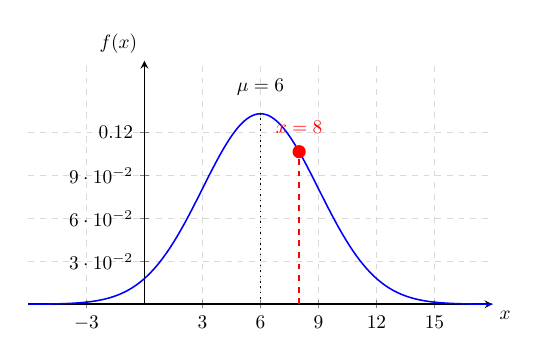
\begin{tikzpicture}[scale=.7]
\begin{axis}[
    width=10cm,
    height=6cm,
    axis lines=center,
    xlabel={$x$},
    ylabel={$f(x)$},
    xlabel style={below right},
    ylabel style={above left},
    xmin=-6, xmax=18,
    ymin=0, ymax=0.17,
    xtick={-3,0,3,6,9,12,15},
    ytick={0,0.03,0.06,0.09,0.12},
    grid=major,
    grid style={dashed,gray!30},
    samples=100,
    smooth,
    thick
]

% Plot the normal distribution with μ=6, σ²=9 (σ=3)
\addplot[blue, thick, domain=-6:18] {1/(3*sqrt(2*pi)) * exp(-0.5*((x-6)/3)^2)};

% Mark x = 8
\addplot[red, thick, mark=*, mark size=3pt] coordinates {(8, {1/(3*sqrt(2*pi)) * exp(-0.5*((8-6)/3)^2)})};

% Draw vertical line at x = 8
\draw[red, thick, dashed] (axis cs:8,0) -- (axis cs:8,{1/(3*sqrt(2*pi)) * exp(-0.5*((8-6)/3)^2)});

% Label the point
\node[red, above] at (axis cs:8,{1/(3*sqrt(2*pi)) * exp(-0.5*((8-6)/3)^2) + 0.008}) {$x = 8$};

% Mark the mean
\draw[black, thick, dotted] (axis cs:6,0) -- (axis cs:6,{1/(3*sqrt(2*pi))});
\node[black, above] at (axis cs:6,{1/(3*sqrt(2*pi)) + 0.008}) {$\mu = 6$};
 
\end{axis}
\end{tikzpicture}
\caption{Normal distribution with $\mu = 6$, $\sigma^2 = 9$, and $x = 8$ indicated}
\label{fig:normal_dist_mu6_var9_x8}
\end{figure}
\end{minipage}\pause\hfill
\begin{minipage}{.45\linewidth}
\begin{figure}[htbp]
\centering
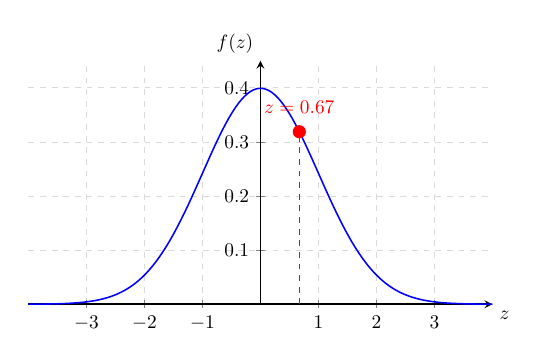
\begin{tikzpicture}[scale=.7]
\begin{axis}[
    width=10cm,
    height=6cm,
    axis lines=center,
    xlabel={$z$},
    ylabel={$f(z)$},
    xlabel style={below right},
    ylabel style={above left},
    xmin=-4, xmax=4,
    ymin=0, ymax=0.45,
    xtick={-3,-2,-1,0,1,2,3},
    ytick={0,0.1,0.2,0.3,0.4},
    grid=major,
    grid style={dashed,gray!30},
    samples=100,
    smooth,
    thick
]

% Plot the standard normal distribution
\addplot[blue, thick, domain=-4:4] {1/sqrt(2*pi) * exp(-0.5*x^2)};

% Mark z = 0.67
\addplot[red, thick, mark=*, mark size=3pt] coordinates {(0.67, {1/sqrt(2*pi) * exp(-0.5*(0.67)^2)})};

% Draw vertical line at z = 0.67
\draw[red, thick, dashed] (axis cs:0.67,0) -- (axis cs:0.67,{1/sqrt(2*pi) * exp(-0.5*(0.67)^2)});

% Label the point
\node[red, above] at (axis cs:0.67,{1/sqrt(2*pi) * exp(-0.5*(0.67)^2) + 0.02}) {$z = 0.67$};

\end{axis}
\end{tikzpicture}
\caption{Standard normal distribution with $z = 0.67$ indicated}
\label{fig:standard_normal_z_0_67}
\end{figure}
\end{minipage}
\end{frame}


\begin{frame}
  \frametitle{Example 4: Finding the normal variate from a $Z$-score}\pause
  A normal r.v.\ $X\sim \mathcal{N}(\mu = 2,\sigma= 3)$ has a $Z$-score of $z = 1.25$. \pause
  What is the corresponding $x$ value? \pause
  \medskip

  
  \begin{minipage}{.48\linewidth}  
    \begin{figure}[htbp]
\centering
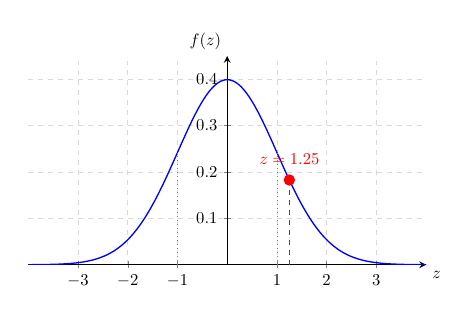
\begin{tikzpicture}[scale=.6]
\begin{axis}[
    width=10cm,
    height=6cm,
    axis lines=center,
    xlabel={$z$},
    ylabel={$f(z)$},
    xlabel style={below right},
    ylabel style={above left},
    xmin=-4, xmax=4,
    ymin=0, ymax=0.45,
    xtick={-3,-2,-1,0,1,2,3},
    ytick={0,0.1,0.2,0.3,0.4},
    grid=major,
    grid style={dashed,gray!30},
    samples=100,
    smooth,
    thick
]

% Plot the standard normal distribution
\addplot[blue, thick, domain=-4:4] {1/sqrt(2*pi) * exp(-0.5*x^2)};

% Mark z = 1.25
\addplot[red, thick, mark=*, mark size=3pt] coordinates {(1.25, {1/sqrt(2*pi) * exp(-0.5*(1.25)^2)})};

% Draw vertical line at z = 1.25
\draw[red, thick, dashed] (axis cs:1.25,0) -- (axis cs:1.25,{1/sqrt(2*pi) * exp(-0.5*(1.25)^2)});

% Label the point
\node[red, above] at (axis cs:1.25,{1/sqrt(2*pi) * exp(-0.5*(1.25)^2) + 0.02}) {$z = 1.25$};

% Mark the mean at z = 0
\draw[black, thick, dotted] (axis cs:0,0) -- (axis cs:0,{1/sqrt(2*pi)});
 
% Add title
 
% Mark standard deviation points for reference
\draw[gray, thin, dotted] (axis cs:-1,0) -- (axis cs:-1,{1/sqrt(2*pi) * exp(-0.5)});
\draw[gray, thin, dotted] (axis cs:1,0) -- (axis cs:1,{1/sqrt(2*pi) * exp(-0.5)});
\node[gray, below] at (axis cs:-1,-0.02) {$-1\sigma$};
\node[gray, below] at (axis cs:1,-0.02) {$+1\sigma$};

\end{axis}
\end{tikzpicture}
\caption{Standard normal distribution with $z = 1.25$ indicated}
\label{fig:standard_normal_z125}
\end{figure}  
  \end{minipage}\pause\hfill
  \begin{minipage}{.48\linewidth}
    \begin{figure}[htbp]
\centering
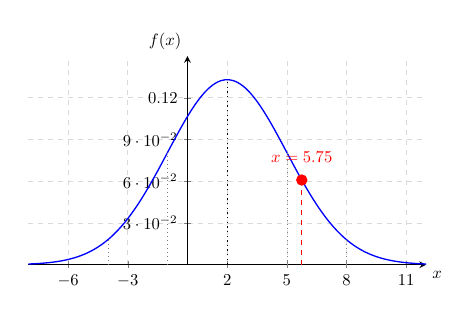
\begin{tikzpicture}[scale=.6]
\begin{axis}[
    width=10cm,
    height=6cm,
    axis lines=center,
    xlabel={$x$},
    ylabel={$f(x)$},
    xlabel style={below right},
    ylabel style={above left},
    xmin=-8, xmax=12,
    ymin=0, ymax=0.15,
    xtick={-6,-3,0,2,5,8,11},
    ytick={0,0.03,0.06,0.09,0.12},
    grid=major,
    grid style={dashed,gray!30},
    samples=100,
    smooth,
    thick
]

% Plot the normal distribution with μ=2, σ=3
\addplot[blue, thick, domain=-8:12] {1/(3*sqrt(2*pi)) * exp(-0.5*((x-2)/3)^2)};

% Mark x = 5.75
\addplot[red, thick, mark=*, mark size=3pt] coordinates {(5.75, {1/(3*sqrt(2*pi)) * exp(-0.5*((5.75-2)/3)^2)})};

% Draw vertical line at x = 5.75
\draw[red, thick, dashed] (axis cs:5.75,0) -- (axis cs:5.75,{1/(3*sqrt(2*pi)) * exp(-0.5*((5.75-2)/3)^2)});

% Label the point
\node[red, above] at (axis cs:5.75,{1/(3*sqrt(2*pi)) * exp(-0.5*((5.75-2)/3)^2) + 0.008}) {$x = 5.75$};

% Mark the mean
\draw[black, thick, dotted] (axis cs:2,0) -- (axis cs:2,{1/(3*sqrt(2*pi))});
%\node[black, above] at (axis cs:2,{1/(3*sqrt(2*pi)) + 0.008}) {$\mu = 2$};

% Add distribution parameters
%\node[above] at (axis cs:2,0.140) {$\mathcal{N}(2, 3^2)$};

% Mark standard deviation points for reference
\draw[gray, thin, dotted] (axis cs:-1,0) -- (axis cs:-1,{1/(3*sqrt(2*pi)) * exp(-0.5)});
\draw[gray, thin, dotted] (axis cs:5,0) -- (axis cs:5,{1/(3*sqrt(2*pi)) * exp(-0.5)});
\draw[gray, thin, dotted] (axis cs:-4,0) -- (axis cs:-4,{1/(3*sqrt(2*pi)) * exp(-2)});
\draw[gray, thin, dotted] (axis cs:8,0) -- (axis cs:8,{1/(3*sqrt(2*pi)) * exp(-2)});

% Labels for standard deviation markers
\node[gray, below] at (axis cs:-1,-0.005) {$\mu-\sigma$};
\node[gray, below] at (axis cs:5,-0.005) {$\mu+\sigma$};
\node[gray, below] at (axis cs:-4,-0.005) {$\mu-2\sigma$};
\node[gray, below] at (axis cs:8,-0.005) {$\mu+2\sigma$};

% Show z-score calculation
%\node[red, font=\small] at (axis cs:8.5,0.08) {$z = \frac{5.75-2}{3} = 1.25$};

\end{axis}
\end{tikzpicture}
\caption{Normal distribution with $\mu = 2$, $\sigma = 3$, and $x = 5.75$ indicated}
\label{fig:normal_mu2_sigma3_x575}
\end{figure}    
  \end{minipage}

  {\gr
    \begin{eqnarray*}
      z &=& \fr{x - \mu}{\sigma} \\\pause
      x &=& \mu + z\sigma = \pause 2 + 1.25(3) = \boxed{5.75}
    \end{eqnarray*}
  }

\end{frame}

\begin{frame}
  \frametitle{68-95-99.7 rule}\pause
      The probabilities of a normal r.v.\ within $\pm1$, $\pm2$ and $\pm3$ standard deviations are
    68.3\%, 95.4\% and 99.7\%, respectively. \pause
    This is known as the \textbf{68-95-99.7 rule} or the \textbf{empirical rule}.
\begin{figure}[htbp]
\centering
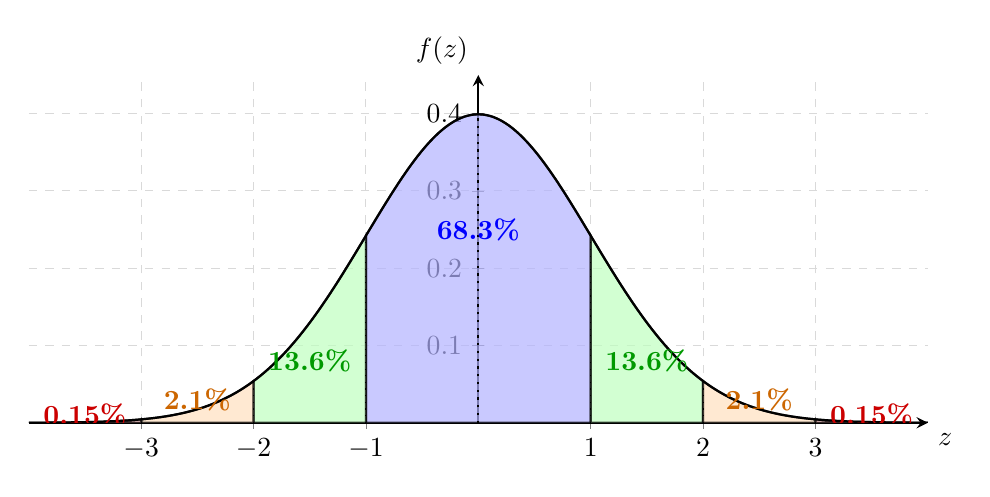
\begin{tikzpicture}
\begin{axis}[
    width=13cm,
    height=6cm,
    axis lines=center,
    xlabel={$z$},
    ylabel={$f(z)$},
    xlabel style={below right},
    ylabel style={above left},
    xmin=-4, xmax=4,
    ymin=0, ymax=0.45,
    xtick={-3,-2,-1,0,1,2,3},
    ytick={0,0.1,0.2,0.3,0.4},
    grid=major,
    grid style={dashed,gray!30},
    samples=100,
    smooth,
    thick
]

% Shade different regions with different colors
% 68% area (within 1 standard deviation) - Blue
\addplot[fill=blue!30, opacity=0.7, domain=-1:1] {1/sqrt(2*pi) * exp(-0.5*x^2)} \closedcycle;

% 95% area (within 2 standard deviations, excluding the 68% area) - Green
\addplot[fill=green!25, opacity=0.7, domain=-2:-1] {1/sqrt(2*pi) * exp(-0.5*x^2)} \closedcycle;
\addplot[fill=green!25, opacity=0.7, domain=1:2] {1/sqrt(2*pi) * exp(-0.5*x^2)} \closedcycle;

% 99.7% area (within 3 standard deviations, excluding the 95% area) - Orange
\addplot[fill=orange!25, opacity=0.7, domain=-3:-2] {1/sqrt(2*pi) * exp(-0.5*x^2)} \closedcycle;
\addplot[fill=orange!25, opacity=0.7, domain=2:3] {1/sqrt(2*pi) * exp(-0.5*x^2)} \closedcycle;

% Extreme tails (beyond 3 standard deviations) - Red
\addplot[fill=red!25, opacity=0.7, domain=-4:-3] {1/sqrt(2*pi) * exp(-0.5*x^2)} \closedcycle;
\addplot[fill=red!25, opacity=0.7, domain=3:4] {1/sqrt(2*pi) * exp(-0.5*x^2)} \closedcycle;

% Plot the standard normal distribution
\addplot[black, thick, domain=-4:4] {1/sqrt(2*pi) * exp(-0.5*x^2)};

% Mark standard deviation points
\draw[black, thin, dotted] (axis cs:-3,0) -- (axis cs:-3,{1/sqrt(2*pi) * exp(-4.5)});
\draw[black, thin, dotted] (axis cs:-2,0) -- (axis cs:-2,{1/sqrt(2*pi) * exp(-2)});
\draw[black, thin, dotted] (axis cs:-1,0) -- (axis cs:-1,{1/sqrt(2*pi) * exp(-0.5)});
\draw[black, thick, dotted] (axis cs:0,0) -- (axis cs:0,{1/sqrt(2*pi)});
\draw[black, thin, dotted] (axis cs:1,0) -- (axis cs:1,{1/sqrt(2*pi) * exp(-0.5)});
\draw[black, thin, dotted] (axis cs:2,0) -- (axis cs:2,{1/sqrt(2*pi) * exp(-2)});
\draw[black, thin, dotted] (axis cs:3,0) -- (axis cs:3,{1/sqrt(2*pi) * exp(-4.5)});

% Labels for z-values
\node[black, below] at (axis cs:0,-0.02) {$0$};
\node[black, below] at (axis cs:-1,-0.02) {$-1$};
\node[black, below] at (axis cs:1,-0.02) {$1$};
\node[black, below] at (axis cs:-2,-0.02) {$-2$};
\node[black, below] at (axis cs:2,-0.02) {$2$};
\node[black, below] at (axis cs:-3,-0.02) {$-3$};
\node[black, below] at (axis cs:3,-0.02) {$3$};

% Probability labels with matching colors
\node[blue, font=\small, font=\bfseries] at (axis cs:0,0.25) {68.3\%};
\node[green!60!black, font=\small, font=\bfseries] at (axis cs:-1.5,0.08) {13.6\%};
\node[green!60!black, font=\small, font=\bfseries] at (axis cs:1.5,0.08) {13.6\%};
\node[orange!80!black, font=\small, font=\bfseries] at (axis cs:-2.5,0.03) {2.1\%};
\node[orange!80!black, font=\small, font=\bfseries] at (axis cs:2.5,0.03) {2.1\%};
\node[red!80!black, font=\tiny, font=\bfseries] at (axis cs:-3.5,0.01) {0.15\%};
\node[red!80!black, font=\tiny, font=\bfseries] at (axis cs:3.5,0.01) {0.15\%};

% Add title
%\node[above] at (axis cs:0,0.42) {\textbf{Standard Normal Distribution: 68-95-99.7 Rule}};

\end{axis}
\end{tikzpicture}
\caption{Standard normal distribution with color-coded regions showing probability percentages}
\label{fig:standard_normal_colored_regions}
\end{figure}
  

\end{frame}

% \begin{frame}
%   \frametitle{Standard deviation of a normal distribution}\pause
%   \begin{minipage}{.4\linewidth}
%     The probabilities of a normal r.v.\ within $\pm1$, $\pm2$ and $\pm3$ standard deviations are
%     68.3\%, 95.4\% and 99.7\%, respectively.    
%   \end{minipage}\quad
%   \begin{minipage}{.55\linewidth}
%     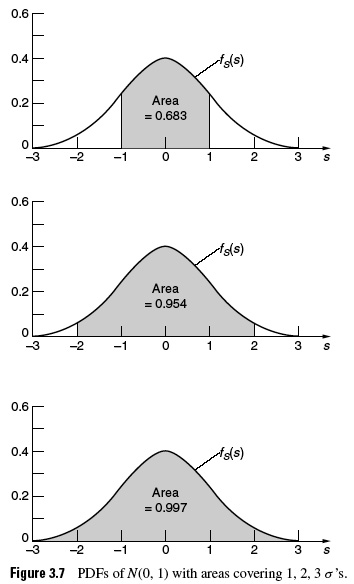
\includegraphics[width=.7\textwidth]{03_07}    
%   \end{minipage}

% \end{frame}



\section{Computing normal probabilities}


\begin{frame}
  \frametitle{Probability of a normal random variable}\pause
  
  The probability that a normal r.v.\ lies within a certain interval is given by the {\it area} under the PDF in that interval. 

  \pause
  
  %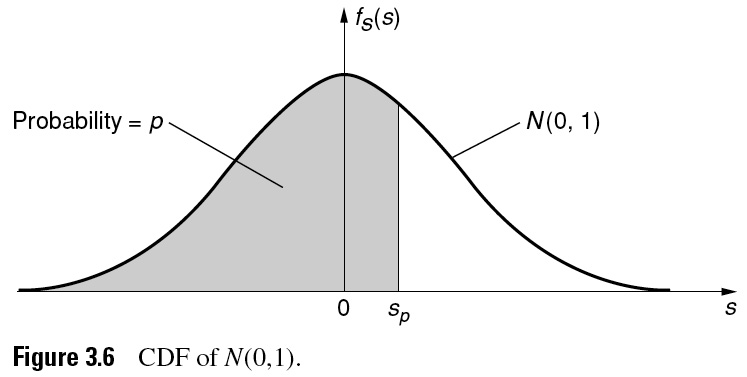
\includegraphics[width=.8\textwidth,trim=0 34 0 0, clip]{03_06}

  \begin{figure}[htbp]
\centering
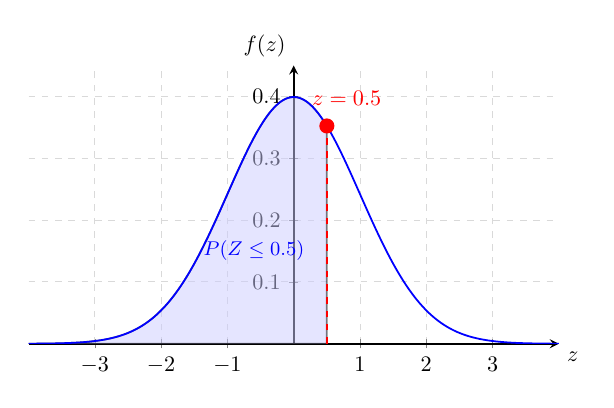
\begin{tikzpicture}[scale=.8]
\begin{axis}[
    width=10cm,
    height=6cm,
    axis lines=center,
    xlabel={$z$},
    ylabel={$f(z)$},
    xlabel style={below right},
    ylabel style={above left},
    xmin=-4, xmax=4,
    ymin=0, ymax=0.45,
    xtick={-3,-2,-1,0,1,2,3},
    ytick={0,0.1,0.2,0.3,0.4},
    grid=major,
    grid style={dashed,gray!30},
    samples=100,
    smooth,
    thick
]

% Shade area to the left of z = 0.5
\addplot[fill=blue!20, opacity=0.5, domain=-4:0.5] {1/sqrt(2*pi) * exp(-0.5*x^2)} \closedcycle;

% Plot the standard normal distribution
\addplot[blue, thick, domain=-4:4] {1/sqrt(2*pi) * exp(-0.5*x^2)};

% Mark z = 0.5
\addplot[red, thick, mark=*, mark size=3pt] coordinates {(0.5, {1/sqrt(2*pi) * exp(-0.5*(0.5)^2)})};

% Draw vertical line at z = 0.5
\draw[red, thick, dashed] (axis cs:0.5,0) -- (axis cs:0.5,{1/sqrt(2*pi) * exp(-0.5*(0.5)^2)});

% Label the point
\node[red, above] at (axis cs:0.8,{1/sqrt(2*pi) * exp(-0.5*(0.5)^2) + 0.02}) {$z = 0.5$};

% Label the shaded area
\node[blue, font=\small] at (axis cs:-.6,0.15) {$P(Z \leq 0.5)$};
%\node[blue, font=\small] at (axis cs:-1.5,0.12) {$\approx 0.6915$};

\end{axis}
\end{tikzpicture}
\caption{Standard normal distribution with $z = 0.5$ indicated and $P(Z \leq 0.5)$ shaded}
\label{fig:standard_normal_z_0_5_shaded}
\end{figure}
  \pause

  \begin{itemize}[<+->]
  \item Recall that the area under the PDF within a given interval is the CDF evaluated in that range
  \item Thus, in the above figure: $p = P(Z \le z_p) = \Phi(z_p)$ %and $z_p = \Phi^{-1}(p)$
  \end{itemize}
\end{frame}

\begin{frame}
  \frametitle{Probability of a normal random variable (cont.)}\pause

  Given a normal r.v.\ $X \sim \mathcal{N}(\mu,\sigma^2)$: \pause

  \begin{equation}
    \label{eq:9}
    P(a < X \le b) = \fr{1}{\sigma\sqrt{2\pi}}\int_a^b e^{-\fr12\lt(\fr{x-\mu}{\sigma}\rt)^2}dx
  \end{equation}

  \pause

  Substituting $z = \fr{x-\mu}{\sigma}$ and $dx = \sigma dz$, we obtain: \pause

  \begin{equation}
    \label{eq:10}
    P(a < X \le b) = \fr{1}{\sqrt{2\pi}}\int_{(a-\mu)/\sigma}^{(b-\mu)/\sigma} e^{-\fr12z^2}dz
  \end{equation}

  \pause

  Recognizing that the integrand is the PDF of a standard normal distribution, we have: \pause

  \begin{equation}
    \label{eq:11} \rd
    P(a < X \le b) =  \Phi\lt(\fr{b-\mu}{\sigma}\rt) -  \Phi\lt(\fr{a-\mu}{\sigma}\rt)
  \end{equation}
\end{frame}

\begin{frame}[fragile]
  \frametitle{Example 5a: Normal probabilities}
  \pause
  SAT scores are normally distributed as $X \sim \mathcal{N}(1100, \sigma=200)$. \pause
  \begin{enumerate}[\bf(a)]
  \item What is the probability that a randomly selected student has a score that is at least 1200? \pause
    {\gr \pause
      The Z-score is $z = \fr{1200 - 1100}{200} = 0.5$ \pause

      Thus,
      \begin{eqnarray*}
      P( X \ge 1200) &=&1 -  \Phi(.5) = \pause 1 - .695 = \boxed{.3085}
      \end{eqnarray*}

    } \pause
\begin{minipage}{.55\linewidth}
In Python, you can compute this probability using the \texttt{scipy.stats} library:      
   \begin{python}
import scipy.stats as stats
p = 1 - stats.norm.cdf(1200, 1100, 200)
  \end{python}
      The first 3 arguments of \texttt{stats.norm.cdf} are the value, mean (texttt{loc}), and standard deviation (texttt{scale}), respectively. \pause
      OR, you can use the $Z$-score (default mean=0, std=1):
       \begin{python}
import scipy.stats as stats
p = 1 - stats.norm.cdf(0.5)
      \end{python}
      \pause which gives the same result.
\end{minipage}
\begin{minipage}{.4\linewidth}
  \begin{figure}[htbp]
\centering
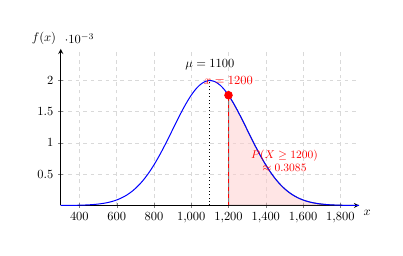
\begin{tikzpicture}[scale=0.45]
\begin{axis}[
    width=10cm,
    height=6cm,
    axis lines=center,
    xlabel={$x$},
    ylabel={$f(x)$},
    xlabel style={below right},
    ylabel style={above left},
    xmin=300, xmax=1900,
    ymin=0, ymax=0.0025,
    xtick={400,600,800,1000,1200,1400,1600,1800},
    ytick={0,0.0005,0.001,0.0015,0.002},
    grid=major,
    grid style={dashed,gray!30},
    samples=100,
    smooth,
    thick
]

% Shade area to the right of x = 1200
\addplot[fill=red!20, opacity=0.5, domain=1200:1900] {1/(200*sqrt(2*pi)) * exp(-0.5*((x-1100)/200)^2)} \closedcycle;

% Plot the normal distribution with μ=1100, σ=200
\addplot[blue, thick, domain=300:1900] {1/(200*sqrt(2*pi)) * exp(-0.5*((x-1100)/200)^2)};

% Mark x = 1200
\addplot[red, thick, mark=*, mark size=3pt] coordinates {(1200, {1/(200*sqrt(2*pi)) * exp(-0.5*((1200-1100)/200)^2)})};

% Draw vertical line at x = 1200
\draw[red, thick, dashed] (axis cs:1200,0) -- (axis cs:1200,{1/(200*sqrt(2*pi)) * exp(-0.5*((1200-1100)/200)^2)});

% Label the point
\node[red, above] at (axis cs:1200,{1/(200*sqrt(2*pi)) * exp(-0.5*((1200-1100)/200)^2) + 0.0001}) {$x = 1200$};

% Mark the mean
\draw[black, thick, dotted] (axis cs:1100,0) -- (axis cs:1100,{1/(200*sqrt(2*pi))});
\node[black, above] at (axis cs:1100,{1/(200*sqrt(2*pi)) + 0.0001}) {$\mu = 1100$};

% Label the shaded area
\node[red, font=\small] at (axis cs:1500,0.0008) {$P(X \geq 1200)$};
\node[red, font=\small] at (axis cs:1500,0.0006) {$\approx 0.3085$};

\end{axis}
\end{tikzpicture}
\end{figure}

  \begin{figure}[htbp]
\centering
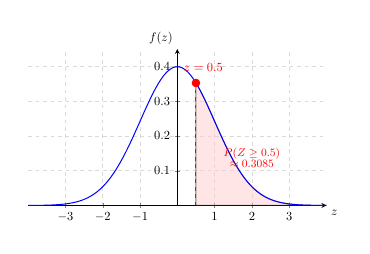
\begin{tikzpicture}[scale=0.45]
\begin{axis}[
    width=10cm,
    height=6cm,
    axis lines=center,
    xlabel={$z$},
    ylabel={$f(z)$},
    xlabel style={below right},
    ylabel style={above left},
    xmin=-4, xmax=4,
    ymin=0, ymax=0.45,
    xtick={-3,-2,-1,0,1,2,3},
    ytick={0,0.1,0.2,0.3,0.4},
    grid=major,
    grid style={dashed,gray!30},
    samples=100,
    smooth,
    thick
]

% Shade area to the right of z = 0.5
\addplot[fill=red!20, opacity=0.5, domain=0.5:4] {1/sqrt(2*pi) * exp(-0.5*x^2)} \closedcycle;

% Plot the standard normal distribution
\addplot[blue, thick, domain=-4:4] {1/sqrt(2*pi) * exp(-0.5*x^2)};

% Mark z = 0.5
\addplot[red, thick, mark=*, mark size=3pt] coordinates {(0.5, {1/sqrt(2*pi) * exp(-0.5*(0.5)^2)})};

% Draw vertical line at z = 0.5
\draw[red, thick, dashed] (axis cs:0.5,0) -- (axis cs:0.5,{1/sqrt(2*pi) * exp(-0.5*(0.5)^2)});

% Label the point
\node[red, above] at (axis cs:0.7,{1/sqrt(2*pi) * exp(-0.5*(0.5)^2) + 0.02}) {$z = 0.5$};

% Label the shaded area
\node[red, font=\small] at (axis cs:2,0.15) {$P(Z \geq 0.5)$};
\node[red, font=\small] at (axis cs:2,0.12) {$\approx 0.3085$};

\end{axis}
\end{tikzpicture}
\end{figure}
\end{minipage}
\end{enumerate}
\end{frame}

\begin{frame}[fragile]
  \frametitle{Example 5b: Normal probabilities}
  \pause
  SAT scores are normally distributed as $X \sim \mathcal{N}(1100, \sigma=200)$. \pause
  \begin{enumerate}[\bf(a)]\setcounter{enumi}{1}
  \item What is the probability that another randomly selected student's score is greater than 600 but less than 1200? \pause
    {\gr \begin{eqnarray*}
           P( 600 \le X < 1200) &=& \Phi\lt( \fr{1200-1100}{200}\rt)  - \Phi\lt( \fr{600-1100}{200}\rt)  \\\pause
                                &=& \Phi(.5) - \Phi(-2.5) \pause
                                = \boxed{.6853}
    \end{eqnarray*}}

\begin{minipage}{.45\linewidth}
In Python:  
\begin{python}
from scipy.stats import norm
p = norm.cdf(1200, 1100, 200) 
    - norm.cdf(600, 1100, 200)
\end{python} \pause
\end{minipage}\pause
\begin{minipage}{.53\linewidth}
\begin{figure}[htbp]
%\centering
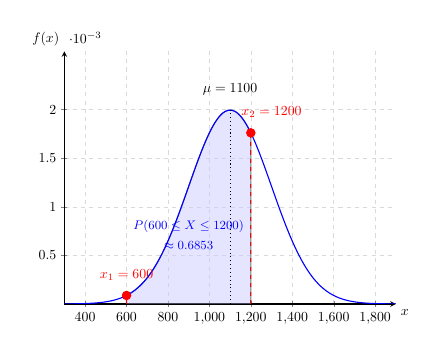
\begin{tikzpicture}[scale=0.5]
\begin{axis}[
    width=10cm,
    height=8cm,
    axis lines=center,
    xlabel={$x$},
    ylabel={$f(x)$},
    xlabel style={below right},
    ylabel style={above left},
    xmin=300, xmax=1900,
    ymin=0, ymax=0.0026,
    xtick={400,600,800,1000,1200,1400,1600,1800},
    ytick={0,0.0005,0.001,0.0015,0.002},
    grid=major,
    grid style={dashed,gray!30},
    samples=100,
    smooth,
    thick
]

% Shade area between x = 600 and x = 1200
\addplot[fill=blue!20, opacity=0.5, domain=600:1200] {1/(200*sqrt(2*pi)) * exp(-0.5*((x-1100)/200)^2)} \closedcycle;

% Plot the normal distribution with μ=1100, σ=200
\addplot[blue, thick, domain=300:1900] {1/(200*sqrt(2*pi)) * exp(-0.5*((x-1100)/200)^2)};

% Mark x = 600
\addplot[red, thick, mark=*, mark size=3pt] coordinates {(600, {1/(200*sqrt(2*pi)) * exp(-0.5*((600-1100)/200)^2)})};

% Mark x = 1200
\addplot[red, thick, mark=*, mark size=3pt] coordinates {(1200, {1/(200*sqrt(2*pi)) * exp(-0.5*((1200-1100)/200)^2)})};

% Draw vertical line at x = 600
\draw[red, thick, dashed] (axis cs:600,0) -- (axis cs:600,{1/(200*sqrt(2*pi)) * exp(-0.5*((600-1100)/200)^2)});

% Draw vertical line at x = 1200
\draw[red, thick, dashed] (axis cs:1200,0) -- (axis cs:1200,{1/(200*sqrt(2*pi)) * exp(-0.5*((1200-1100)/200)^2)});

% Label the points
\node[red, above] at (axis cs:600,{1/(200*sqrt(2*pi)) * exp(-0.5*((600-1100)/200)^2) + 0.0001}) {$x_1 = 600$};
\node[red, above] at (axis cs:1300,{1/(200*sqrt(2*pi)) * exp(-0.5*((1200-1100)/200)^2) + 0.0001}) {$x_2 = 1200$};

% Mark the mean
\draw[black, thick, dotted] (axis cs:1100,0) -- (axis cs:1100,{1/(200*sqrt(2*pi))});
\node[black, above] at (axis cs:1100,{1/(200*sqrt(2*pi)) + 0.0001}) {$\mu = 1100$};

% Label the shaded area
\node[blue, font=\small] at (axis cs:900,0.0008) {$P(600 \leq X \leq 1200)$};
\node[blue, font=\small] at (axis cs:900,0.0006) {$\approx 0.6853$};

\end{axis}
\end{tikzpicture}
\end{figure}

\end{minipage}

\end{enumerate}
\end{frame}


\begin{frame}[fragile]
  \frametitle{Example 5b: Normal probabilities (cont)}
  \pause
  \begin{enumerate}[\bf(a)]\setcounter{enumi}{1}
  \item OR, you can use the $Z$-scores (default mean=0, std=1):
\begin{python}
import scipy.stats as stats
p = norm.cdf(0.5) - norm.cdf(-2.5)
\end{python}

\begin{minipage}{.48\linewidth}  
\begin{figure}[htbp]
\centering
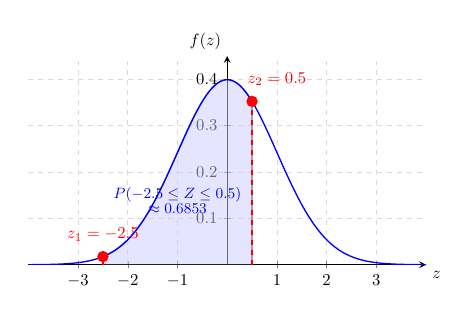
\begin{tikzpicture}[scale=0.6]
\begin{axis}[
    width=10cm,
    height=6cm,
    axis lines=center,
    xlabel={$z$},
    ylabel={$f(z)$},
    xlabel style={below right},
    ylabel style={above left},
    xmin=-4, xmax=4,
    ymin=0, ymax=0.45,
    xtick={-3,-2,-1,0,1,2,3},
    ytick={0,0.1,0.2,0.3,0.4},
    grid=major,
    grid style={dashed,gray!30},
    samples=100,
    smooth,
    thick
]

% Shade area between z = -2.5 and z = 0.5
\addplot[fill=blue!20, opacity=0.5, domain=-2.5:0.5] {1/sqrt(2*pi) * exp(-0.5*x^2)} \closedcycle;

% Plot the standard normal distribution
\addplot[blue, thick, domain=-4:4] {1/sqrt(2*pi) * exp(-0.5*x^2)};

% Mark z = -2.5
\addplot[red, thick, mark=*, mark size=3pt] coordinates {(-2.5, {1/sqrt(2*pi) * exp(-0.5*(-2.5)^2)})};

% Mark z = 0.5
\addplot[red, thick, mark=*, mark size=3pt] coordinates {(0.5, {1/sqrt(2*pi) * exp(-0.5*(0.5)^2)})};

% Draw vertical line at z = -2.5
\draw[red, thick, dashed] (axis cs:-2.5,0) -- (axis cs:-2.5,{1/sqrt(2*pi) * exp(-0.5*(-2.5)^2)});

% Draw vertical line at z = 0.5
\draw[red, thick, dashed] (axis cs:0.5,0) -- (axis cs:0.5,{1/sqrt(2*pi) * exp(-0.5*(0.5)^2)});

% Label the points
\node[red, above] at (axis cs:-2.5,{1/sqrt(2*pi) * exp(-0.5*(-2.5)^2) + 0.02}) {$z_1 = -2.5$};
\node[red, above] at (axis cs:1,{1/sqrt(2*pi) * exp(-0.5*(0.5)^2) + 0.02}) {$z_2 = 0.5$};

% Label the shaded area
\node[blue, font=\small] at (axis cs:-1,0.15) {$P(-2.5 \leq Z \leq 0.5)$};
\node[blue, font=\small] at (axis cs:-1,0.12) {$\approx 0.6853$};

\end{axis}
\end{tikzpicture}
\caption{Standard normal PDF with probability area shaded}
\end{figure}
\end{minipage}\pause\hfill
\begin{minipage}{.48\linewidth}  
\begin{figure}[htbp]
\centering  
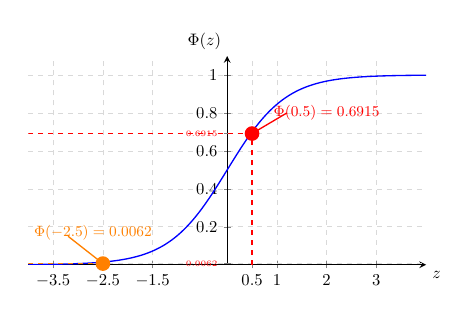
\begin{tikzpicture}[scale=.6]
\begin{axis}[
    width=10cm,
    height=6cm,
    axis lines=center,
    xlabel={$z$},
    ylabel={$\Phi(z)$},
    xlabel style={below right},
    ylabel style={above left},
    xmin=-4, xmax=4,
    ymin=0, ymax=1.1,
    xtick={-3.5,-2.5,-1.5,0,0.5, 1,2,3},
    ytick={0,0.2,0.4,0.6,0.8,1.0},
    extra y ticks={0.0062, 0.6915},
    extra y tick labels={0.0062, 0.6915},
    extra y tick style={grid=major, tick label style={font=\tiny, red}},
    grid=major,
    grid style={dashed,gray!30},
    samples=200,
    smooth,
    thick
]

% Plot the standard normal CDF using sigmoid approximation
\addplot[blue, thick, domain=-4:4] {1/(1 + exp(-1.7*x))};

% For z = 0.5: Φ(0.5) ≈ 0.6915
\draw[red, thick, dashed] (axis cs:-4,0.6915) -- (axis cs:0.5,0.6915);
\draw[red, thick, dashed] (axis cs:0.5,0) -- (axis cs:0.5,0.6915);
\addplot[red, thick, mark=*, mark size=4pt] coordinates {(0.5, 0.6915)};

% For z = -2.5: Φ(-2.5) ≈ 0.0062
\draw[orange, thick, dashed] (axis cs:-4,0.0062) -- (axis cs:-2.5,0.0062);
\draw[orange, thick, dashed] (axis cs:-2.5,0) -- (axis cs:-2.5,0.0062);
\addplot[orange, thick, mark=*, mark size=4pt] coordinates {(-2.5, 0.0062)};

% Clean labels
\node[red, font=\small] at (axis cs:2,0.8) {$\Phi(0.5) = 0.6915$};
\node[orange, font=\small] at (axis cs:-2.7,0.17) {$\Phi(-2.5) = 0.0062$};

% Arrows pointing to the values
\draw[red, ->, thick] (axis cs:1.2,0.8) -- (axis cs:0.5,0.6915);
\draw[orange, ->, thick] (axis cs:-3.2,0.15) -- (axis cs:-2.5,0.0062);

\end{axis}
\end{tikzpicture}
\caption{Standard normal CDF with corresponding probability values marked}
\label{fig:standard_normal_cdf_specific}
\end{figure}
\end{minipage}
%\end{figure}
 
\end{enumerate}
\end{frame}

\begin{frame}[fragile]
  \frametitle{Example 6: Inverse normal probabilities}
  \pause
  SAT scores are normally distributed as $X \sim \mathcal{N}(1100, \sigma=200)$. \pause
  \begin{enumerate}[\bf(a)]\setcounter{enumi}{2}
  \item If the probability of an SAT score lower than $x$ is 0.4, find $x$. \pause
    {\gr \pause
      \begin{eqnarray*}
        z &=& \Phi^{-1}(.4) = -.2533 = \fr{x-\mu}{\sigma} \\\pause 
        \therefore x &=& z\sigma + \mu = -.2533(200) + 1100 = \boxed{1049}
      \end{eqnarray*}

    } \pause
\begin{python}
from scipy.stats import norm
p = norm.ppf(0.4, 1100, 200)
\end{python}
\pause
  \begin{figure}[htbp]
\centering
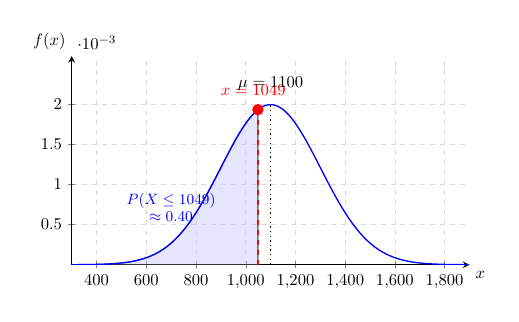
\begin{tikzpicture}[scale=.6]
\begin{axis}[
    width=10cm,
    height=6cm,
    axis lines=center,
    xlabel={$x$},
    ylabel={$f(x)$},
    xlabel style={below right},
    ylabel style={above left},
    xmin=300, xmax=1900,
    ymin=0, ymax=0.0026,
    xtick={400,600,800,1000,1200,1400,1600,1800},
    ytick={0,0.0005,0.001,0.0015,0.002},
    grid=major,
    grid style={dashed,gray!30},
    samples=100,
    smooth,
    thick
]

% Shade area to the left of x = 1049
\addplot[fill=blue!20, opacity=0.5, domain=300:1049] {1/(200*sqrt(2*pi)) * exp(-0.5*((x-1100)/200)^2)} \closedcycle;

% Plot the normal distribution with μ=1100, σ=200
\addplot[blue, thick, domain=300:1900] {1/(200*sqrt(2*pi)) * exp(-0.5*((x-1100)/200)^2)};

% Mark x = 1049
\addplot[red, thick, mark=*, mark size=3pt] coordinates {(1049, {1/(200*sqrt(2*pi)) * exp(-0.5*((1049-1100)/200)^2)})};

% Draw vertical line at x = 1049
\draw[red, thick, dashed] (axis cs:1049,0) -- (axis cs:1049,{1/(200*sqrt(2*pi)) * exp(-0.5*((1049-1100)/200)^2)});

% Label the point
\node[red, above] at (axis cs:1030,{1/(200*sqrt(2*pi)) * exp(-0.5*((1049-1100)/200)^2) + 0.0001}) {$x = 1049$};

% Mark the mean
\draw[black, thick, dotted] (axis cs:1100,0) -- (axis cs:1100,{1/(200*sqrt(2*pi))});
\node[black, above] at (axis cs:1100,{1/(200*sqrt(2*pi)) + 0.0001}) {$\mu = 1100$};

% Label the shaded area
\node[blue, font=\small] at (axis cs:700,0.0008) {$P(X \leq 1049)$};
\node[blue, font=\small] at (axis cs:700,0.0006) {$\approx 0.40$};

\end{axis}
\end{tikzpicture}
\caption{Normal distribution with $\mu = 1100$, $\sigma = 200$, and $P(X \leq 1049)$ shaded}
\label{fig:normal_dist_mu1100_sigma200_x1049}
\end{figure}

  \end{enumerate}
\end{frame}

\begin{frame}[fragile]
  \frametitle{Example 6: Inverse normal probabilities (cont.)}
  \pause
  \begin{enumerate}[\bf(a)]\setcounter{enumi}{2}
  \item You can think of the inverse CDF as finding the $x$ value that corresponds to a given percentile. \pause
\begin{figure}[htbp]
\centering
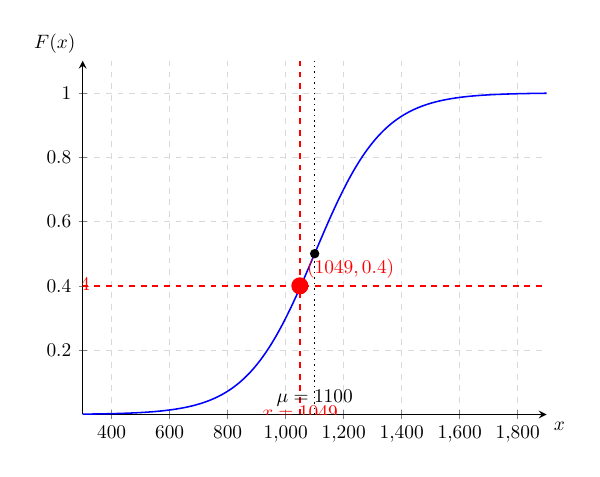
\begin{tikzpicture}[scale=.7]
\begin{axis}[
    width=10cm,
    height=8cm,
    axis lines=center,
    xlabel={$x$},
    ylabel={$F(x)$},
    xlabel style={below right},
    ylabel style={above left},
    xmin=300, xmax=1900,
    ymin=0, ymax=1.1,
    xtick={400,600,800,1000,1200,1400,1600,1800},
    ytick={0,0.2,0.4,0.6,0.8,1.0},
    grid=major,
    grid style={dashed,gray!30},
    samples=200,
    smooth,
    thick
]

% Plot normal CDF using sigmoid approximation for better accuracy
\addplot[blue, thick, domain=300:1900] {1/(1 + exp(-1.7*(x-1100)/200))};

% Draw horizontal line at y = 0.4
\draw[red, thick, dashed] (axis cs:300,0.4) -- (axis cs:1900,0.4);

% Draw vertical line at x = 1049
\draw[red, thick, dashed] (axis cs:1049,0) -- (axis cs:1049,1.1);

% Mark the intersection point
\addplot[red, thick, mark=*, mark size=4pt] coordinates {(1049, 0.4)};

% Label the intersection point
\node[red, above right] at (axis cs:1049,0.4) {$(1049, 0.4)$};

% Label the lines
\node[red, left] at (axis cs:350,0.4) {$F(1049) = 0.4$};
\node[red, below] at (axis cs:1049,0.05) {$x = 1049$};

% Mark the mean (where F(μ) = 0.5)
\draw[black, thick, dotted] (axis cs:1100,0) -- (axis cs:1100,1.1);
\node[black, below] at (axis cs:1100,0.1) {$\mu = 1100$};
\addplot[black, mark=*, mark size=2pt] coordinates {(1100, 0.5)};

\end{axis}
\end{tikzpicture}
\caption{Normal distribution CDF showing the 40th percentile at $x = 1049$}
\label{fig:normal_cdf_percentile}
\end{figure}
  \end{enumerate}
\end{frame}

\begin{frame}
  \frametitle{More on the normal CDF}\pause
  
  %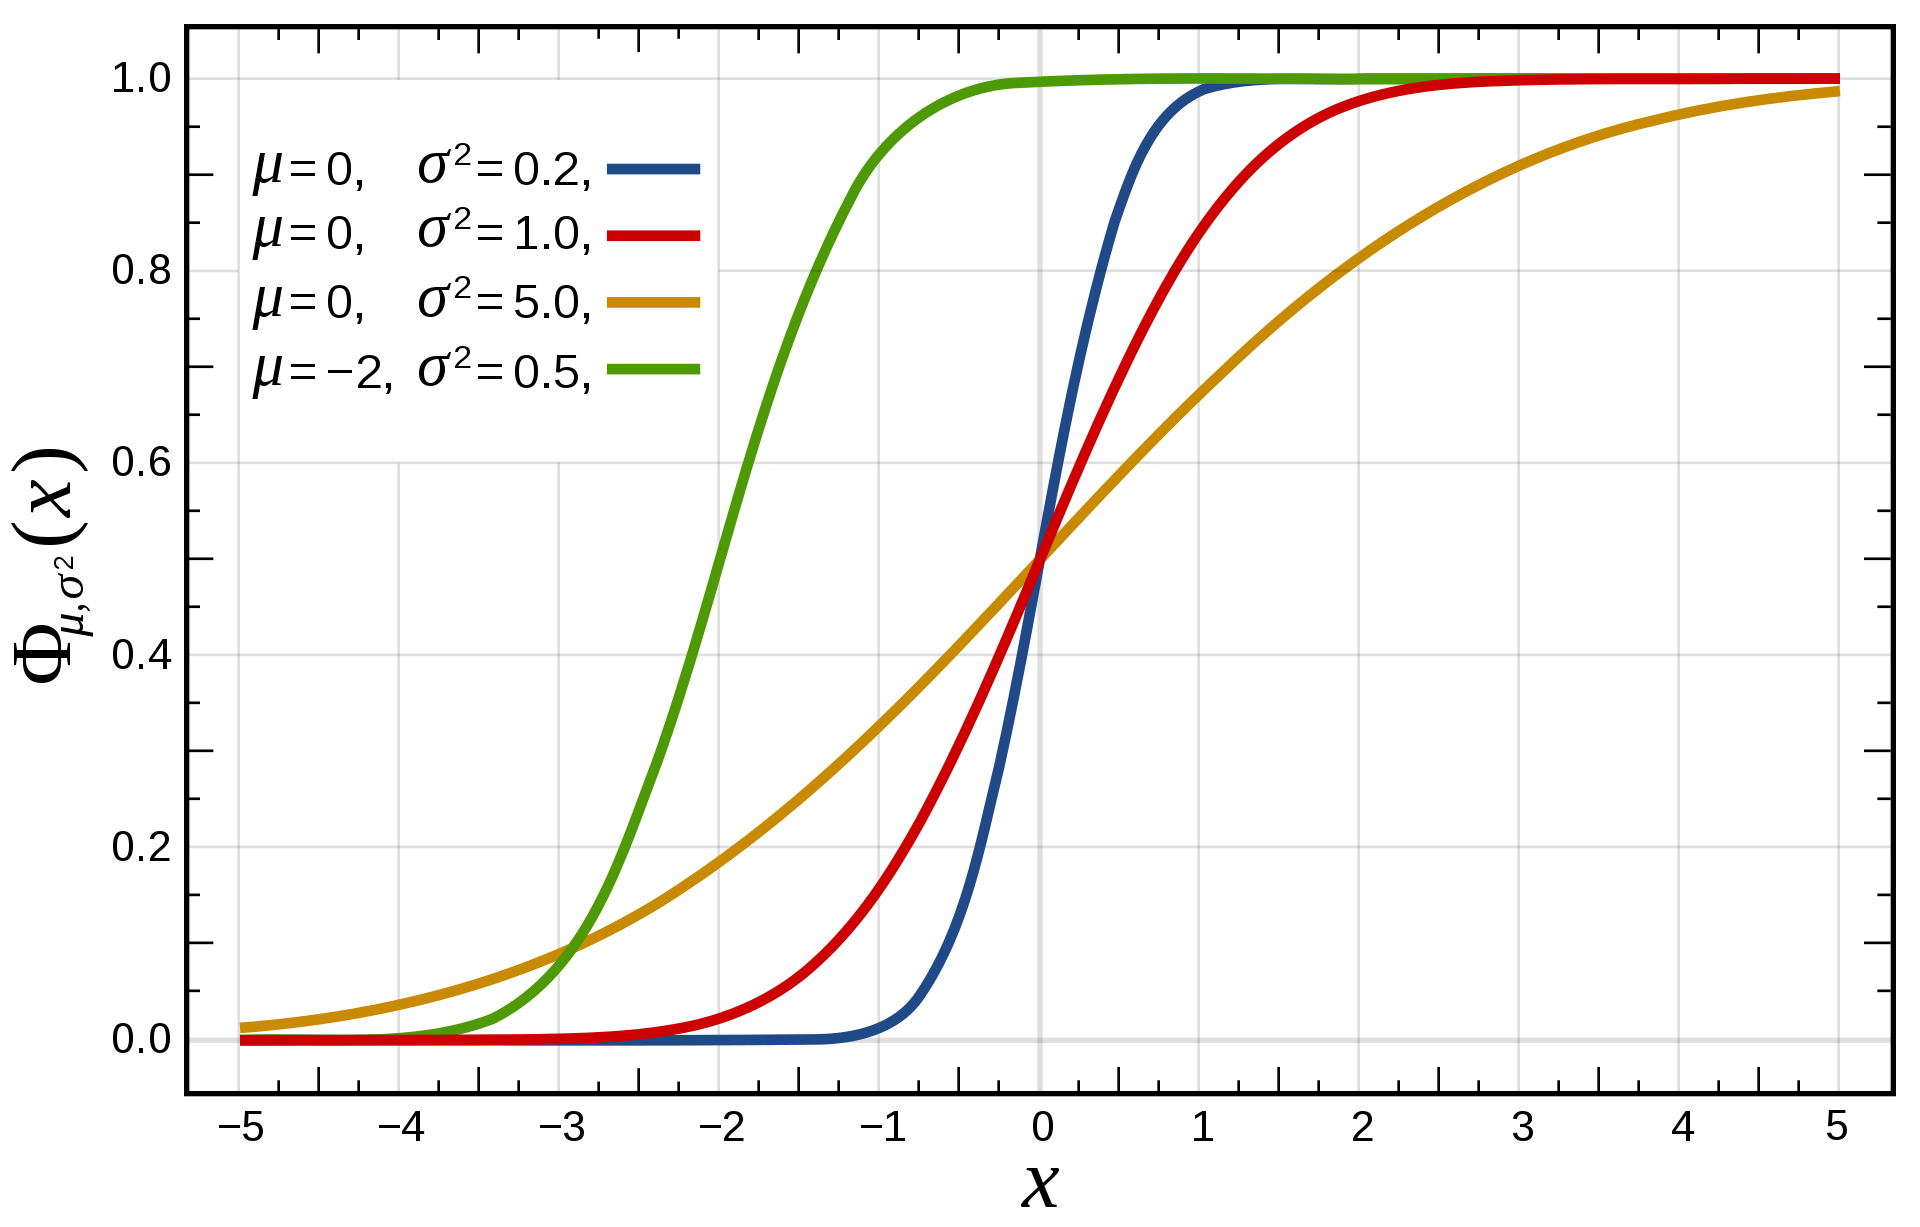
\includegraphics[width=.7\textwidth]{normdist-cdf}

  \begin{figure}[htbp]
\centering
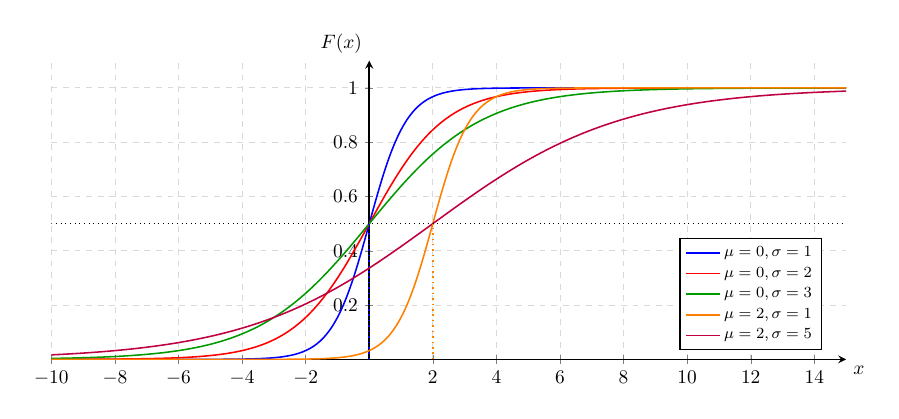
\begin{tikzpicture}[scale=.7]
\begin{axis}[
    width=16cm,
    height=7cm,
    axis lines=center,
    xlabel={$x$},
    ylabel={$F(x)$},
    xlabel style={below right},
    ylabel style={above left},
    xmin=-10, xmax=15,
    ymin=0, ymax=1.1,
    xtick={-12, -10, -8,-6,-4,-2,0,2,4,6,8,10,12,14, 16},
    ytick={0,0.2,0.4,0.6,0.8,1.0},
    grid=major,
    grid style={dashed,gray!30},
    samples=200,
    smooth,
    thick,
    legend pos=south east,
    legend style={font=\footnotesize}
]

% 1. mu = 0, sd = 1 (Standard normal)
\addplot[blue, thick, domain=-10:15] {1/(1 + exp(-1.7*(x-0)/1))};
\addlegendentry{$\mu = 0, \sigma = 1$}

% 2. mu = 0, sd = 2
\addplot[red, thick, domain=-10:15] {1/(1 + exp(-1.7*(x-0)/2))};
\addlegendentry{$\mu = 0, \sigma = 2$}

% 3. mu = 0, sd = 3
\addplot[green!60!black, thick, domain=-10:15] {1/(1 + exp(-1.7*(x-0)/3))};
\addlegendentry{$\mu = 0, \sigma = 3$}

% 4. mu = 2, sd = 1
\addplot[orange, thick, domain=-10:15] {1/(1 + exp(-1.7*(x-2)/1))};
\addlegendentry{$\mu = 2, \sigma = 1$}

% 5. mu = 2, sd = 5
\addplot[purple, thick, domain=-10:15] {1/(1 + exp(-1.7*(x-2)/5))};
\addlegendentry{$\mu = 2, \sigma = 5$}

% Mark the means with vertical dotted lines
\draw[blue, dotted, thick] (axis cs:0,0) -- (axis cs:0,0.5);
\draw[orange, dotted, thick] (axis cs:2,0) -- (axis cs:2,0.5);

% Add horizontal line at 0.5 for reference
\draw[black, dotted, thin] (axis cs:-10,0.5) -- (axis cs:15,0.5);

% Label the means
\node[blue, below] at (axis cs:0,-0.05) {$\mu_1 = 0$};
\node[orange, below] at (axis cs:2,-0.05) {$\mu_2 = 2$};

% Add title
%\node[above] at (axis cs:2.5,1.05) {\textbf{Comparison of Normal CDFs}};

\end{axis}
\end{tikzpicture}
\caption{Comparison of normal distribution CDFs with different parameters}
\label{fig:normal_cdf_comparison}
\end{figure}
  \pause

  \begin{itemize}[<+->]
  \item The standard normal CDF is the blue curve in the above figure
  \item Quantiles can be read off the plot (e.g.\ the median is the value of $X$ corresponding to the $y$ value of 0.5)
  \item $\Phi(-z) = 1 - \Phi(z)$
  \item $z = \Phi^{-1}(p) = - \Phi^{-1}(1-p)$
  \end{itemize}
\end{frame}

\section{More Examples}
\begin{frame}
  \frametitle{Example 7: Probability of flooding}\pause
    The drainage from a community during a storm is a normal random variable
    estimated to have a mean of 1.2 million gallons per day (mgd) and an SD of
    0.4 mgd. If the storm drain system is designed with a maximum drainage
    capacity of 1.5 mgd:
    \begin{enumerate}[\bf(a)]\pause
    \item What is the underlying probability of flooding during  a storm that is assumed in the design of the drainage system?
    \item Find $P(1.0 < X \le 1.6)$.
    \item Find the 90th-percentile drainage load from the community during a storm.
    \end{enumerate}
 \end{frame}


\begin{frame}
  \frametitle{Example 7: Probability of flooding (cont.)}
    \pause
    Given $\mu = 1.2$ and $\sigma = 0.4$. \pause
    \begin{enumerate}[\bf(a)]
    \item What is the underlying probability of flooding during  a storm that is assumed in the design of the drainage system?

      \pause
      \begin{exampleblock}{Solution} \pause

\begin{minipage}{.48\linewidth}
          \begin{figure}[htbp]
\centering
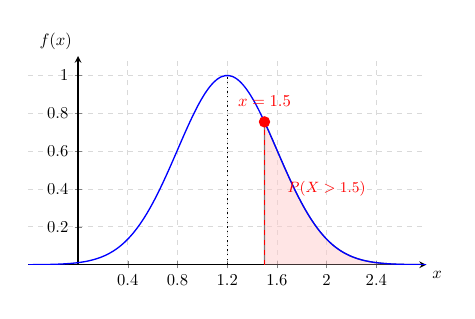
\begin{tikzpicture}[scale=.6]
\begin{axis}[
    width=10cm,
    height=6cm,
    axis lines=center,
    xlabel={$x$},
    ylabel={$f(x)$},
    xlabel style={below right},
    ylabel style={above left},
    xmin=-0.4, xmax=2.8,
    ymin=0, ymax=1.1,
    xtick={0,0.4,0.8,1.2,1.6,2.0,2.4},
    ytick={0,0.2,0.4,0.6,0.8,1.0},
    grid=major,
    grid style={dashed,gray!30},
    samples=100,
    smooth,
    thick
]

% Shade area to the right of x = 1.5
\addplot[fill=red!20, opacity=0.5, domain=1.5:2.8] {1/(0.4*sqrt(2*pi)) * exp(-0.5*((x-1.2)/0.4)^2)} \closedcycle;

% Plot the normal distribution with μ=1.2, σ=0.4
\addplot[blue, thick, domain=-0.4:2.8] {1/(0.4*sqrt(2*pi)) * exp(-0.5*((x-1.2)/0.4)^2)};

% Mark x = 1.5
\addplot[red, thick, mark=*, mark size=3pt] coordinates {(1.5, {1/(0.4*sqrt(2*pi)) * exp(-0.5*((1.5-1.2)/0.4)^2)})};

% Draw vertical line at x = 1.5
\draw[red, thick, dashed] (axis cs:1.5,0) -- (axis cs:1.5,{1/(0.4*sqrt(2*pi)) * exp(-0.5*((1.5-1.2)/0.4)^2)});

% Label the point
\node[red, above] at (axis cs:1.5,{1/(0.4*sqrt(2*pi)) * exp(-0.5*((1.5-1.2)/0.4)^2) + 0.05}) {$x = 1.5$};

% Mark the mean
\draw[black, thick, dotted] (axis cs:1.2,0) -- (axis cs:1.2,{1/(0.4*sqrt(2*pi))});
%\node[black, above] at (axis cs:1.2,{1/(0.4*sqrt(2*pi)) + 0.05}) {$\mu = 1.2$};

% Label the shaded area
\node[red, font=\small] at (axis cs:2.0,0.4) {$P(X > 1.5)$};
%\node[red, font=\small] at (axis cs:2.0,0.32) {$\approx 0.227$};

% Add distribution parameters
%\node[above] at (axis cs:1.2,1.05) {$\mu = 1.2, \sigma = 0.4$};

\end{axis}
\end{tikzpicture}
\caption{Normal distribution with $\mu = 1.2$, $\sigma = 0.4$, and $P(X > 1.5)$ shaded}
\label{fig:normal_dist_mu1_2_sigma0_4_x1_5}
\end{figure}
\end{minipage}\pause\hfill
\begin{minipage}{.48\linewidth}
      \begin{eqnarray*}
      P(X > 1.5) &=& 1 - P(X \le 1.5) \\ \pause
                 &=& 1 - \Phi\lt(\fr{1.5 - 1.2}{0.4}\rt) \\  \pause
                 &=& 1 - \Phi(0.75) \\ \pause
                 &=& 1 - 0.7734 = \boxed{0.227}
    \end{eqnarray*}
    \pause
    In Python: \pythoninline{1 - norm.cdf(1.5, 1.2, 0.4)}
\end{minipage}
  \end{exampleblock}

    \end{enumerate}
 \end{frame}


\begin{frame}
  \frametitle{Example 7: Probability of flooding (cont.)}\pause
    \begin{enumerate}[\bf(a)]\setcounter{enumi}{1}
    \item Find $p = P(1.0 < X \le 1.6)$: \pause

        \begin{exampleblock}{Solution}\pause
\begin{minipage}{.43\linewidth}
          \begin{figure}[htbp]
\centering
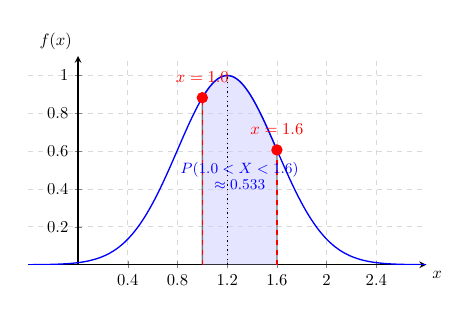
\begin{tikzpicture}[scale=.6]
\begin{axis}[
    width=10cm,
    height=6cm,
    axis lines=center,
    xlabel={$x$},
    ylabel={$f(x)$},
    xlabel style={below right},
    ylabel style={above left},
    xmin=-0.4, xmax=2.8,
    ymin=0, ymax=1.1,
    xtick={0,0.4,0.8,1.2,1.6,2.0,2.4},
    ytick={0,0.2,0.4,0.6,0.8,1.0},
    grid=major,
    grid style={dashed,gray!30},
    samples=100,
    smooth,
    thick
]

% Shade area between x = 1.0 and x = 1.6
\addplot[fill=blue!20, opacity=0.5, domain=1.0:1.6] {1/(0.4*sqrt(2*pi)) * exp(-0.5*((x-1.2)/0.4)^2)} \closedcycle;

% Plot the normal distribution with μ=1.2, σ=0.4
\addplot[blue, thick, domain=-0.4:2.8] {1/(0.4*sqrt(2*pi)) * exp(-0.5*((x-1.2)/0.4)^2)};

% Mark x = 1.0
\addplot[red, thick, mark=*, mark size=3pt] coordinates {(1.0, {1/(0.4*sqrt(2*pi)) * exp(-0.5*((1.0-1.2)/0.4)^2)})};

% Mark x = 1.6
\addplot[red, thick, mark=*, mark size=3pt] coordinates {(1.6, {1/(0.4*sqrt(2*pi)) * exp(-0.5*((1.6-1.2)/0.4)^2)})};

% Draw vertical line at x = 1.0
\draw[red, thick, dashed] (axis cs:1.0,0) -- (axis cs:1.0,{1/(0.4*sqrt(2*pi)) * exp(-0.5*((1.0-1.2)/0.4)^2)});

% Draw vertical line at x = 1.6
\draw[red, thick, dashed] (axis cs:1.6,0) -- (axis cs:1.6,{1/(0.4*sqrt(2*pi)) * exp(-0.5*((1.6-1.2)/0.4)^2)});

% Label the points
\node[red, above] at (axis cs:1.0,{1/(0.4*sqrt(2*pi)) * exp(-0.5*((1.0-1.2)/0.4)^2) + 0.05}) {$x = 1.0$};
\node[red, above] at (axis cs:1.6,{1/(0.4*sqrt(2*pi)) * exp(-0.5*((1.6-1.2)/0.4)^2) + 0.05}) {$x = 1.6$};

% Mark the mean
\draw[black, thick, dotted] (axis cs:1.2,0) -- (axis cs:1.2,{1/(0.4*sqrt(2*pi))});
%\node[black, above] at (axis cs:1.2,{1/(0.4*sqrt(2*pi)) + 0.05}) {$\mu = 1.2$};

% Label the shaded area
\node[blue, font=\small] at (axis cs:1.3,0.5) {$P(1.0 < X < 1.6)$};
\node[blue, font=\small] at (axis cs:1.3,0.42) {$\approx 0.533$};

% Add distribution parameters
%\node[above] at (axis cs:1.2,1.05) {$\mu = 1.2, \sigma = 0.4$};

\end{axis}
\end{tikzpicture}
\caption{Normal distribution with $\mu = 1.2$, $\sigma = 0.4$, and $P(1.0 < X < 1.6)$ shaded}
\label{fig:normal_dist_mu1_2_sigma0_4_interval}
\end{figure}
\end{minipage}  \pause
\begin{minipage}{.53\linewidth}
                \begin{eqnarray*}
          p &=& \Phi\lt(\fr{1.6 -1.2}{0.4} \rt) \\
          && \quad - \Phi\lt(\fr{1.0 - 1.2}{0.4}\rt) \\\pause
                           &=& \Phi(1.0) - \Phi(-0.5) \\ \pause
                           &=& 0.8413 - [1 - \Phi(0.5)] \\ \pause
                           &=& 0.8413 - (1- 0.6915)\\\pause
                           &=& 0.8413 - 0.3085\\\pause
                           &=& 0.5328 \approx \boxed{0.533}
      \end{eqnarray*}
      \end{minipage}          
      \pause
      \medskip
      In Python: \pythoninline{norm.cdf(1.6, 1.2, 0.4) - norm.cdf(1.0, 1.2, 0.4)}
\end{exampleblock}

    \end{enumerate}
 \end{frame}

\begin{frame}
  \frametitle{Example 7: Probability of flooding (cont.)} \pause
    \begin{enumerate}[\bf(a)]\setcounter{enumi}{2}
    \item Find the 90th-percentile drainage load from the community during a storm. \pause


        \begin{figure}[htbp]
\centering
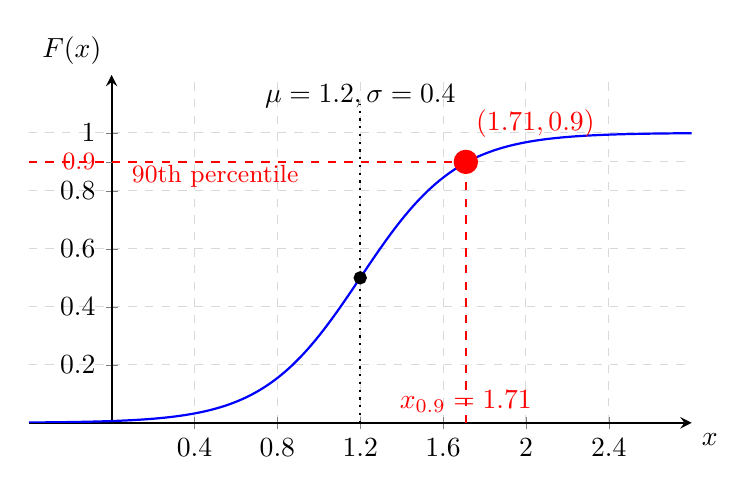
\begin{tikzpicture}
\begin{axis}[
    width=10cm,
    height=6cm,
    axis lines=center,
    xlabel={$x$},
    ylabel={$F(x)$},
    xlabel style={below right},
    ylabel style={above left},
    xmin=-0.4, xmax=2.8,
    ymin=0, ymax=1.2,
    xtick={0,0.4,0.8,1.2,1.6,2.0,2.4},
    ytick={0,0.2,0.4,0.6,0.8,1.0},
    extra y ticks={0.9},
    extra y tick labels={0.9},
    extra y tick style={grid=major, tick label style={font=\small, red}},
    %extra x ticks={1.71},
    %extra x tick labels={1.71},
    %extra x tick style={grid=major, tick label style={font=\small, red}},
    grid=major,
    grid style={dashed,gray!30},
    samples=200,
    smooth,
    thick
]

% Plot the normal CDF with μ=1.2, σ=0.4
% Using sigmoid approximation: F(x) ≈ 1/(1 + exp(-1.7*(x-μ)/σ))
\addplot[blue, thick, domain=-0.4:2.8] {1/(1 + exp(-1.7*(x-1.2)/0.4))};

% Draw horizontal line at y = 0.9
\draw[red, thick, dashed] (axis cs:-0.4,0.9) -- (axis cs:1.71,0.9);

% Draw vertical line at x = 1.71
\draw[red, thick, dashed] (axis cs:1.71,0) -- (axis cs:1.71,0.9);

% Mark the intersection point
\addplot[red, thick, mark=*, mark size=4pt] coordinates {(1.71, 0.9)};

% Label the intersection point
\node[red, above right] at (axis cs:1.71,.95) {$(1.71, 0.9)$};

% Labels on axes
%\node[red, left] at (axis cs:-0.2,0.9) {$P = 0.9$};
\node[red, above] at (axis cs:1.71,0) {$x_{0.9} = 1.71$};

% Mark the mean (where F(μ) = 0.5)
\draw[black, thick, dotted] (axis cs:1.2,0) -- (axis cs:1.2,1.1);
\node[black, below] at (axis cs:1.2,-0.05) {$\mu = 1.2$};
\addplot[black, mark=*, mark size=2pt] coordinates {(1.2, 0.5)};

% Add distribution parameters and interpretation
\node[above] at (axis cs:1.2,1.05) {$\mu = 1.2, \sigma = 0.4$};
\node[red, font=\small] at (axis cs:0.5,0.85) {90th percentile};

\end{axis}
\end{tikzpicture}
\caption{Normal CDF showing the 90th percentile at $x = 1.71$}
\label{fig:normal_cdf_90th_percentile}
\end{figure}
  
    \end{enumerate}
 \end{frame}

\begin{frame}[fragile]
  \frametitle{Example 7: Probability of flooding (cont.)} \pause
    \begin{enumerate}[(a)]\setcounter{enumi}{2}
    \item Find the 90th-percentile drainage load from the community during a storm. \pause

      \begin{exampleblock}{Solution}
\pause
      \begin{eqnarray*}
        P(X\le x_{0.90}) \pause &=& \Phi\lt( \fr{x_{0.90} - 1.2}{0.40}\rt) = 0.90 \\ \pause
        \implies \fr{x_{0.90} - 1.2}{0.40}\pause  &=& \Phi^{-1}(0.90) \pause = 1.28 \\ \pause
        \therefore x_{0.90} \pause &=& 1.28(0.40) + 1.2 = \pause 1.71 \text{ mgd}
      \end{eqnarray*}
      \pause
      In Python:
      \begin{python}
from scipy.stats import norm
p90 = norm.ppf(0.9, 1.2, 0.4)
      \end{python}
      gives 1.7095 mgd
    \end{exampleblock}

    \end{enumerate}
 \end{frame}

\begin{frame}
  \frametitle{Example 8: Steel beam reliability} \pause Assume the
    variability $E$ in the lengths of steel beams is normally distributed. What
    is the precision (in terms of $\sigma$) required for a reliability of
    99.7\%, given that the specified tolerance for a construction project is
    $\pm 5$ mm?\pause

    \medskip

    Definitions:
    \begin{itemize}[<+->]
      \item \textbf{Precision}: in physical terms is the inverse of the variance (i.e.\ higher precision means lower variance). In this context, all you need to do is find the standard deviation $\sigma$.
    \item \textbf{Reliability}: probability that the deviation in the length of a beam meets (falls within) the specified tolerance
    \end{itemize}

  %   \begin{exampleblock}{Solution}\pause
  %   \begin{eqnarray*}
  %     P(-5 \le E \le 5) &=& \Phi\lt(\fr{5-0}{\sigma}\rt) - \Phi\lt(\fr{-5-0}{\sigma}\rt) = 0.997\\ \pause
  %     2\Phi\lt(\fr{5}{\sigma}\rt) - 1 &=& 0.997 \\ \pause
  %     \Phi\lt(\fr{5}{\sigma}\rt)  &=& \fr{1 + 0.997}{2} = 0.9985 \\ \pause
  %     \fr{5}{\sigma} &=& \Phi^{-1}(0.9985) = \pause 2.97 \\ \pause
  %     \implies \text{The required precision is: } \sigma &=& \pause \boxed{1.68 \text{ mm}}
  %   \end{eqnarray*}
  % \end{exampleblock}

    
\end{frame}

\section{Outlook}


\begin{frame}
  \frametitle{Recap of normal distribution}
  \pause

  \begin{itemize}
  \item The {\gr PDF} of the normal distribution (parameters $\mu$ and $\sigma^{2}$) is given by \pause
    \begin{equation}\gr
      f_{X}(x) = \fr{1}{\sigma\sqrt{2\pi}}\exp\lt[\fr{1}{2}\lt(\fr{x - \mu}{\sigma}\rt)^{2}\rt]
    \end{equation}

  \item  The parameters of a normal distribution $\mathcal{N}(\mu,\sigma^{2})$ correspond to its mean and variance, respectively.
    \pause
    
  \item There is no closed-form solution to the integral of the normal CDF
    \pause
    
  \item Instead, it is customary to standardize a normal variable to its {\bl ``Z-score''}:\pause
    \begin{equation}\bl
      Z = \fr{X - \mu}{\sigma}
    \end{equation}
    \pause
  \item The mean and variance of the standard normal distribution are 0 and 1, respectively.
    \pause
    
  \item The symbol {\og $\Phi$ (``phi'')} is used to represent the CDF of the {\og \textit{standard} normal distribution}, whose
    values can be looked up in a table.
    \pause
    
  \item In Python, the \texttt{\rd scipy.stats.norm.cdf(x, mu, sigma)} and \texttt{\rd scipy.stats.norm.ppf(p, mu, sigma)} can be used to compute
    probabilities and inverse CDFs of the normal distribution, respectively.
  \end{itemize}
\end{frame}
%\begin{frame}[allowframebreaks]
%   \frametitle{References}
%   \AtNextBibliography{\scriptsize}
%   \setbeamertemplate{bibliography item}[text]
%   \printbibliography[heading=none]
  
% \end{frame}

%\printbibliography
\end{document}
%%% Local Variables:
%%% mode: latex
%%% TeX-master: t
%%% End:
